%  LaTeX support: latex@mdpi.com 
%  For support, please attach all files needed for compiling as well as the log file, and specify your operating system, LaTeX version, and LaTeX editor.
%
%  manuscript_v3.tex: internal bibliography (MDPI template variant B, ACS format for Mathematics).
%  References are embedded below; biblio.bib is not required at compile time.
%  To refresh entries after citation changes: compile v2 with BibTeX and copy manuscript_v2.bbl.

%=================================================================
\documentclass[mathematics,article,submit,moreauthors]{Definitions/mdpi} 

%=================================================================
% MDPI internal commands - do not modify
\firstpage{1} 
\makeatletter 
\setcounter{page}{\@firstpage}
\makeatother
\pubvolume{1}
\issuenum{1}
\articlenumber{0}
\pubyear{2026}
\copyrightyear{2026} 
%\externaleditor{Firstname Lastname} % More than 1 editor, please add `` and '' before the last editor name
\datereceived{ } 
\daterevised{ } % Comment out if no revised date
\dateaccepted{ } 
\datepublished{ } 
%\datecorrected{} % For corrected papers: "Corrected: XXX" date in the original paper.
%\dateretracted{} % For retracted papers: "Retracted: XXX" date in the original paper.
%\doinum{} % Used for some special journals, like molbank
%\pdfoutput=1 % Uncommented for upload to arXiv.org
%\CorrStatement{yes}  % For updates
%\longauthorlist{yes} % For many authors that exceed the left citation part
%\IsAssociation{yes} % For association journals

%=================================================================
% Add packages and commands here. The following packages are loaded in our class file: fontenc, inputenc, calc, indentfirst, fancyhdr, graphicx, epstopdf, lastpage, ifthen, float, amsmath, amssymb, lineno, setspace, enumitem, mathpazo, booktabs, titlesec, etoolbox, tabto, xcolor, colortbl, soul, multirow, microtype, tikz, totcount, changepage, attrib, upgreek, array, tabularx, pbox, ragged2e, tocloft, marginnote, marginfix, enotez, amsthm, natbib, hyperref, cleveref, scrextend, url, geometry, newfloat, caption, draftwatermark, seqsplit
% cleveref: load \crefname definitions after \begin{document}

\usepackage{xcolor}

%=================================================================
% Please use the following mathematics environments: Theorem, Lemma, Corollary, Proposition, Characterization, Property, Problem, Example, ExamplesandDefinitions, Hypothesis, Remark, Definition, Notation, Assumption
%% For proofs, please use the proof environment (the amsthm package is loaded by the MDPI class).

%=================================================================
% Full title of the paper (Capitalized)


\Title{Aggregation Semantics for Prioritization in Cooperative Automated Decision Making}

% Author Orchid ID: enter ID or remove command 
\newcommand{\orcidauthorA}{0000-0003-3267-6753} % Add \orcidA{} behind the author's name
\newcommand{\orcidauthorB}{0009-0002-0183-7905} % Add \orcidB{} behind the author's name
\newcommand{\orcidauthorC}{0000-0002-7653-1452} % Add \orcidB{} behind the author's name

% Authors, for the paper (add full first names)
\Author{Pavel Novoa-Hern\'andez$^{1,*}$\orcidA{}, Mariia Godz$^{2}$\orcidA{} and David A. Pelta$^{2}$\orcidC{}}

%\longauthorlist{yes}

% MDPI internal command: Authors, for metadata in PDF
\AuthorNames{Pavel Novoa-Hern\'andez, Mariia Godz and David A. Pelta}

%\longauthorlist{yes}

% Affiliations / Addresses (Add [1] after \address if there is only one affiliation.)
\address{%
$^{1}$ \quad Dept. Computer Engineering and Systems, Universidad de La Laguna; pnovoahe@ull.edu.es\\
$^{2}$ \quad Dept. Computer Science and Artificial Intelligence, Universidad de Granada; \{mariiagodz,dpelta\}@ugr.es}

% Contact information of the corresponding author
\corres{Correspondence:pnovoahe@ull.edu.es}

% Current address and/or shared authorship
%\firstnote{Current address: Affiliation.}  
% Current address should not be the same as any items in the Affiliation section.

%\secondnote{These authors contributed equally to this work.}
% The commands \thirdnote{} till \eighthnote{} are available for further notes.

%\simplesumm{} % Simple summary

%\conference{} % An extended version of a conference paper

% Abstract (Do not insert blank lines, i.e. \\) 
\abstract{%{\color{blue}Hybrid automated decision-making systems increasingly combine predictive outputs from machine-learning models with contextual knowledge, organizational policies, or domain constraints. 
Cooperative Automated Decision-Making Systems (CADEMAS) combine the output of several automated decision making units (the so called predictive evidence) with contextual knowledge, organizational policies, or domain constraints, to produce a robust decision.
Within CADEMAS, the aggregation operator responsible of such combination of information is not merely a mathematical component but the mechanism that defines how predictive evidence and contextual information are reconciled into a final prioritization. This paper investigates the influence of aggregation semantics by comparing the standard linear operator with two well-established alternatives: the conjunctive minimum and the weighted geometric mean. We first derive theoretical conditions characterizing rank reversals and predictive rank preservation under different aggregation regimes. These properties are then examined through Monte Carlo simulations covering policy compliance, predictive overconfidence, and uncertainty in contextual assessments. The results show that linear aggregation provides a flexible trade-off between prediction and context, but may prioritize contextually excluded alternatives when predictive evidence dominates. In contrast, the non-linear operators better preserve contextual constraints and exhibit greater robustness to predictive overconfidence and contextual uncertainty. A realistic employee attrition case study based on a CADEMAS-ML instantiation confirms that these theoretical and simulation results remain visible in practice. Overall, the findings demonstrate that the choice of aggregation operator constitutes a governance decision that directly determines the decision semantics of cooperative automated decision-making systems.}%}

% Keywords
\keyword{
cooperative automated decision making;
aggregation operators;
%fuzzy aggregation;
multi-criteria decision making;
context-aware decision support;
prioritization
}

%%%%%%%%%%%%%%%%%%%%%%%%%%%%%%%%%%%%%%%%%%
\begin{document}


\section{Introduction}

Artificial Intelligence and machine learning techniques, in particular, have improved the ability to estimate risks and anticipate events, in many decision making scenarios. 
However, a good prediction is not always an actionable or good decision. A hospital, a company, or a public agency may need to respect resource limits, institutional policies, safety constraints, or expert-defined priorities before acting on a model output. This is why many decision-support systems are moving from purely predictive pipelines toward hybrid architectures that combine data-driven evidence with rules, contextual information, and domain knowledge \citep{Kierner2023,Rahman2025,PerezDominguez2024}.

This shift creates a methodological problem that is easy to overlook. Once predictive evidence and contextual knowledge coexist, the final recommendation depends on how both signals are integrated. The aggregation rule therefore becomes part of the decision policy. It decides whether a high predicted risk or confidence can compensate for weak contextual support, whether a contextual veto must dominate the model, or whether the system should operate somewhere between those two extremes.


Recently, \citet{NovoaHernandez2026} proposed the Cooperative Automated Decision-Making System (CADEMAS) framework to make this separation explicit. Here, an automated decision-making (ADM) system is regarded as ``a (computational) process, including AI techniques and approaches, that, fed by inputs and data received or collected from the environment, can generate, given a set of predefined objectives, outputs in a wide variety of forms (content, ratings, recommendations, decisions, predictions, etc.)'' \cite{ELI_ADM_Principles_2022}. CADEMAS organizes heterogeneous ADM units within a layered architecture: predictive or automated components produce partial evidence, an integration layer combines their outputs, and a contextual modulator evaluates the result under organizational or institutional criteria.

CADEMAS examples are those presented in \citep{NovoaHernandez2026, Godz2026}. In both cases, the system uses machine learning based ADM with fuzzy rule based context representation. In the former, the aim is to prioritize a set of small and medium enterprises to rescue, whereas in the latter, the aim is to prioritize retention strategies for avoiding employees in attrition risk. In this case, 
fuzzy contextual rules encode retention priorities such as strategic fit, development potential, or organizational vulnerability.

These cases combine predictive score and context through a linear convex rule. The appeal is clear: the parameter is interpretable, and the final score is easy to explain. However, linearity also imposes a strong assumption. It treats prediction or scoring and context as fully compensatory dimensions. For instance, a sufficiently high risk score may offset poor contextual compatibility, and strong contextual support may offset weak predictive evidence. This is not necessarily wrong, but it may be undesirable. In domains where contextual information represents a regulation, a safety requirement, or a fairness constraint, unrestricted compensation may lead to recommendations that are numerically plausible but institutionally unacceptable.

The Multi-Criteria Decision-Making (MCDM) literature, including fuzzy MCDM, offers many alternatives to such basic linear aggregation mechanism. Ordered weighted \citep{Yager1988}, geometric \citep{Tan2009}, t-norm-based \citep{Grabisch1996}, Frank \citep{Riaz2022}, Aczel--Alsina \citep{Senapati2022}, Dombi \citep{Akram2020}, and so on operators have been developed to represent different forms of interaction among criteria for different types of information. 

This literature is mathematically rich and methodologically diverse \citep{Mardani2018,Sun2018,Kahraman2015,Mardani2015}. It characterizes aggregation operators in terms of formal properties, behavioral patterns, extension mechanisms, and parameterized forms that govern how criteria interactions are modeled \citep{Sun2018}. It also shows that the choice of aggregation operator significantly affects criteria weights and the final ranking of alternatives in applied decision problems \citep{Petrovic2023}.


Despite this extensive body of work, aggregation operators have been studied primarily as mathematical constructs or as components of individual decision-making methods. Comparatively less attention has been paid to their role within CADEMAS, where aggregation is responsible for reconciling the outputs of heterogeneous ADM units with contextual or organizational knowledge. In such settings, the aggregation operator is not merely a numerical device; it determines how different sources of evidence interact and, therefore, embodies an implicit decision policy.

This perspective is particularly relevant for the CADEMAS framework. By explicitly separating evidence generation from contextual assessment, CADEMAS allows different aggregation strategies to be applied without modifying the underlying ADM units or the contextual knowledge itself. Consequently, the aggregation mechanism becomes a key design choice: different operators may produce substantially different recommendations or decisions from exactly the same inputs. A highly compensatory strategy may allow strong evidence from one source to outweigh weak contextual support, whereas a more restrictive strategy may preserve contextual constraints even when the automated evidence is highly favorable. The choice of aggregation therefore influences not only numerical scores but also the transparency, robustness, and governance characteristics of the overall decision process.

{\color{red}
Although the mathematical properties of aggregation operators have been extensively studied in fuzzy logic and MCDM, their role as policy-enforcement mechanisms within hybrid Automated Decision-Making architectures remains largely unexplored. Most existing context-aware frameworks, such as those proposed by \citet{Afzal2018} and \citet{Shyur2025}, either treat aggregation as a static numerical step or embed contextual knowledge directly into the predictive process. Consequently, aggregation is rarely analyzed as an independent design component that governs how predictive evidence and contextual information interact.

This limitation is particularly relevant in cooperative decision-making systems such as CADEMAS. In these architectures, the aggregation operator is not merely a numerical device but an implicit decision policy that determines the extent to which predictive evidence can compensate for contextual constraints, or vice versa. Yet, despite the rich body of aggregation research, most studies focus on proposing new operators or demonstrating their usefulness in specific application domains. Comparatively little attention has been paid to understanding how alternative aggregation semantics affect the behavior of an entire cooperative decision-making framework. Questions such as policy compliance, robustness to predictive overconfidence, sensitivity to localized prediction errors, and ranking stability under different aggregation regimes remain largely unexplored. By explicitly separating evidence generation from contextual assessment, CADEMAS provides an ideal setting to isolate aggregation as a modular policy lever and systematically study its effects, distinguishing this work from traditional comparative applications of aggregation operators such as \citet{Blancas2024}.
}

%Surprisingly, this question has received relatively little systematic attention. Although the fuzzy MCDM literature offers a rich collection of aggregation operators and analyzes many of their mathematical properties, most studies focus either on proposing new operators or on demonstrating their usefulness in specific application domains. Comparatively few works investigate how alternative aggregation semantics affect the behavior of an entire cooperative decision-making framework. Questions such as the robustness of prioritization under contextual uncertainty, the sensitivity of recommendations to local predictive errors, or the consistency of resource-allocation policies across different aggregation strategies remain largely unexplored.

This paper addresses this gap in the context of CADEMAS, using as example a prioritization task. Rather than proposing yet another aggregation operator, we investigate how representative aggregation strategies with different compensation semantics influence the behavior of the same cooperative decision-making architecture. Our objective is to understand how the choice of aggregation affects prioritization outcomes, policy compliance, robustness to predictive perturbations, and ranking stability, while preserving the modular philosophy of CADEMAS, in which evidence generation and decision integration remain conceptually independent.

To this end, we combine controlled simulation experiments with the prior CADEMAS example on  employee-attrition introduced by \citet{Godz2026}. The simulation study isolates the effects of aggregation under different operating conditions, whereas the real case study illustrates how these behaviors translate into a practical prioritization scenario. Together, these complementary analyses provide both controlled evidence and application-oriented insight into the implications of aggregation design choices.

The main contributions of this work are as follows:

\begin{itemize}
\item We reinterpret aggregation within CADEMAS as a policy-design mechanism governing the interaction between the outputs of heterogeneous ADM units and contextual knowledge.

\item We compare representative aggregation regimes exhibiting different compensation semantics within a common cooperative decision-making framework.

\item We provide a systematic experimental evaluation of how aggregation semantics affect prioritization behavior, policy compliance, robustness to localized predictive perturbations, and ranking stability.

\item We demonstrate these effects through controlled simulation and a CADEMAS-ML employee-attrition case study, highlighting practical implications of aggregation design choices.

\end{itemize}

The remainder of the paper is organized as follows. Section~\ref{sect:cademas} introduces the CADEMAS framework and its instantiations. Section~\ref{sect:aggregation_operators} formalizes the aggregation models and their structural properties. Section~\ref{sect:simulation} presents the simulation study and its findings. Section~\ref{sect:real_example} applies the operators to a published employee-attrition instantiation. Section~\ref{sect:conclusions} summarizes the main conclusions, limitations, and directions for future work.

\section{The CADEMAS Framework and Its Instantiations}
\label{sect:cademas} 

%\textbf{EN ALGUN LADO TENDRIAMOS QUE MENCIONAR ALGO MÁS DEL CONTEXTO Y CITAR NUESTRO PAPER}

\citet{NovoaHernandez2026} introduced CADEMAS as a general framework for designing context-aware decision-support systems in which multiple heterogeneous Automated Decision-Making (ADM) units cooperate to produce a unified recommendation, score or label. The framework is intentionally independent of the internal nature of these decision units: an ADM may correspond to a predictive model, a rule-based system, an optimization algorithm, an expert system, or any other computational mechanism capable of producing decision evidence. 
Likewise, contextual knowledge may be represented through expert rules, organizational policies, regulatory constraints, or alternative knowledge-representation formalisms.

Rather than prescribing how individual decisions are obtained, CADEMAS defines an architectural process through which heterogeneous decision signals are coordinated and subsequently governed by \textit{contextual} knowledge before a final recommendation is produced.

Formally, a CADEMAS instance is represented by the tuple
\begin{equation}
\mathcal{S}=
\langle I, U, O, K, T \rangle,
\end{equation}
where $I$ denotes the Input Manager, $U$ the set of ADM units, $O$ the Decision Integration Layer, $K$ the Contextual Modulator, and $T$ the universe of admissible data representations. %The framework intentionally abstracts away from the internal implementation of these components. %Consequently, an ADM unit may correspond to a machine-learning model, a rule-based system, an optimization module, or any other computational mechanism capable of producing decision evidence. Likewise, contextual knowledge may be represented through expert rules, organizational policies, regulatory constraints, or alternative knowledge-representation formalisms.

The resulting architecture follows a layered decision process. First, the ADM units independently generate decision evidence from the available input information. Each ADM may rely on a different subset of the available information. The Contextual Modulator, using again all or a part of the input information, produces a ``degree of satisfaction'' with the domain knowledge, organizational priorities, regulatory requirements, or other contextual considerations. 
Finally, the Decision Integration Layer combines the predictive evidence with the contextual's satisfaction degree into a unified decision score. 

This separation between evidence generation and contextual governance is one of the defining characteristics of CADEMAS and enables the same architecture to be instantiated across diverse application domains without modifying its overall decision process.

One important specialization of this framework is the so called CADEMAS-ML, in which the ADM units correspond to machine-learning predictive models. In this case, the predictive subsystem resembles an ensemble architecture in which multiple predictive models cooperate to produce a unified predictive assessment. However, unlike conventional ensemble methods, CADEMAS-ML explicitly separates predictive cooperation from contextual governance. Predictive evidence is first consolidated into a cooperative predictive score and only afterwards, reconciled with \textit{fuzzy} contextual knowledge that encodes organizational or institutional priorities.  This contextual knowledge is represented through a fuzzy inference system inspired by  \citet{PerezCanedo2022} and \citet{PerezCanedo2024}, enabling organizational and institutional priorities to be incorporated in an interpretable manner.

To better illustrate the main ideas of this contribution, in what follows we focus exclusively on CADEMAS-ML. Regardless of the application domain, we abstract the predictive subsystem as a normalized cooperative
\emph{predictive score}
\begin{equation}
R_i \in [0,1],
\end{equation}
which summarizes the collective evidence generated by the cooperating ADM units for decision case $i$. The precise semantics of $R_i$ depend on the application: it may represent, for example, a cooperative risk score, a confidence score, or another normalized predictive assessment.

Independently, the contextual subsystem computes a normalized contextual satisfaction degree
\begin{equation}
Q_i \in [0,1],
\end{equation}
also referred to as the \emph{context score}, which quantifies the extent to which decision case $i$ satisfies the rules of the context.

The predictive and contextual assessments are subsequently combined through an aggregation operator $A$
\begin{equation}
P_i = A(R_i,Q_i),
\end{equation}
to obtain a final \textit{prioritization} score. As we are dealing with a prioritization example, $P_i$ will be used to rank candidate cases and obtain the corresponding Top-$K$ candidates.

Existing CADEMAS-ML applications employ a \textit{linear} convex aggregation operator to combine predictive scores and contextual information. However, the CADEMAS framework itself does not prescribe any particular aggregation semantics \citep{NovoaHernandez2026}. The integration operator can therefore be regarded as an independent design component that determines how predictive scores and contextual knowledge interact. The remainder of this paper investigates alternative aggregation operators and analyzes how their semantics reshape the resulting prioritization process while preserving the overall CADEMAS-ML architecture.


\section{Aggregation Operators for Integrating Predictive Score and Context}
\label{sect:aggregation_operators}

This section formalizes the integration stage of CADEMAS-ML, where the cooperative predictive score and the contextual assessment are combined into a single prioritization score. Rather than restricting the integration mechanism to the linear convex combination employed in previous CADEMAS-ML applications, we consider a broader family of aggregation operators inspired by fuzzy logic and MCDM. This general formulation enables different integration semantics to be analyzed within a common mathematical framework.

Let
\[
A:[0,1]^2 \rightarrow [0,1]
\]
denote an aggregation operator mapping the cooperative predictive score $R_i$ and the contextual assessment $Q_i$ into the final prioritization score
\[
P_i = A(R_i,Q_i).
\]

{\color{red}
Throughout this work, we assume that all aggregation operators satisfy the following basic properties:

\begin{itemize}
\item \textit{Monotonicity:} if $R_i\le R_j$ and $Q_i\le Q_j$, then
\[
A(R_i,Q_i)\le A(R_j,Q_j).
\]
\item \textit{Boundary conditions (Normalization):}
\[
A(0,0)=0,\qquad A(1,1)=1.
\]
\end{itemize}

These properties are standard in fuzzy aggregation and ensure that the operator preserves the natural ordering of inputs and respects the extremes of the unit interval. For the theoretical results in Section~\ref{subsect:rank_properties}, we additionally assume continuity and strict monotonicity in each argument when required. The specific operators considered in this paper satisfy the following additional properties:

\begin{itemize}
\item The linear operator $A_L$ is continuous, strictly increasing in both arguments (for $\lambda\in(0,1)$), and idempotent. It is only commutative in the symmetric case ($\lambda=0.5$). It satisfies $A_L(r,0)>0$ for $r>0$.

\item The minimum $A_C^{\min}$ is continuous, idempotent, commutative, and non-decreasing (though not strictly increasing in general). It satisfies $A_C^{\min}(r,0)=0$ and $A_C^{\min}(r,q)>0$ for $r,q>0$.

\item The algebraic product $A_C^{\prod}$ is continuous, strictly increasing for $r,q>0$, and commutative, but not idempotent. It also satisfies $A_C^{\prod}(r,0)=0$ and $A_C^{\prod}(r,q)>0$ for $r,q>0$.

\item The weighted geometric mean $A_G$ is continuous, strictly increasing for $r,q>0$, and idempotent. Like the linear operator, it is commutative only when $\lambda=0.5$. It satisfies $A_G(r,0)=0$ (for $\lambda\in(0,1)$) and $A_G(r,q)>0$ for $r,q>0$.
\end{itemize}
}

The linear operator corresponds to the integration mechanism adopted in previous CADEMAS-ML implementations and serves as the reference model throughout this work. The remaining operators represent alternative integration policies with progressively different compensation behavior between predictive evidence and contextual information.

\subsection{Linear Aggregation: The Current CADEMAS-ML Integration Scheme}
\label{subsect:linear}

The linear aggregation operator,
\begin{equation}
A_L(R_i,Q_i)=\lambda R_i+(1-\lambda)Q_i,\qquad \lambda\in[0,1],
\end{equation}
corresponds to the integration mechanism adopted in current CADEMAS-ML applications. The parameter $\lambda$ determines the relative importance assigned to the cooperative predictive score ($R_i$) and the contextual assessment ($Q_i$), yielding the final priority score
\[
P_i=A_L(R_i,Q_i).
\]

The operator $A_L$ is fully compensatory. Consider two candidates $i$ and $j$ such that $R_i>R_j$ but $Q_i<Q_j$. Under linear aggregation, their relative ordering depends solely on the value of $\lambda$: any decrease in contextual assessment can always be offset by a sufficiently large increase in predictive score, and vice versa. Consequently, an alternative with weak contextual support may still be prioritized if its predictive performance is sufficiently high.

This compensatory behavior follows directly from the constant partial derivatives
\[
\frac{\partial A_L}{\partial R_i}=\lambda,\qquad
\frac{\partial A_L}{\partial Q_i}=1-\lambda,
\]
which imply a constant marginal rate of substitution between prediction and context. Equivalently, the iso-priority contours in the $(R_i,Q_i)$ plane are straight lines, reflecting the same trade-off throughout the entire score domain. As a result, contextual deficiencies remain fully compensable regardless of their severity.

Although such behavior is appropriate when prediction and context represent equally substitutable sources of information, it may be undesirable in decision scenarios where contextual information encodes safety requirements, fairness constraints, regulatory compliance, or institutional vetoes. In these settings, unrestricted compensation may assign high priority to alternatives that should instead be penalized or excluded from consideration.

\subsection{Alternative Aggregation Operators}
\label{subsect:alternative_operators}

Beyond the linear operator $A_L$, we consider aggregation operators representing different degrees of compensation between predictive evidence and contextual assessment. These operators are well established in fuzzy aggregation and MCDM, and each induces a distinct integration policy within CADEMAS-ML.

\begin{enumerate}

\item \emph{Conjunctive (non-compensatory) aggregation.}
Classical fuzzy conjunction is represented by operators such as the minimum and the algebraic product \citep{Zimmermann1980}:
\begin{equation}
A_C^{\min}(R_i,Q_i)=\min(R_i,Q_i),
\end{equation}
\begin{equation}
A_C^{\prod}(R_i,Q_i)=R_iQ_i.
\end{equation}

Both operators prevent full compensation between prediction and context. Under the minimum operator, the final priority cannot exceed the weaker component, so a poor contextual assessment directly limits the overall score. In particular, if $Q_i=0$, then $P_i=0$ regardless of the predictive score, naturally implementing an institutional veto. This interpretation is consistent with the role of non-compensatory aggregation in composite indicators and policy evaluation \citep{Natoli2024,Blancas2024}. The algebraic product shares the same zero-absorption property while providing a smoother penalization of intermediate values than the minimum.

For completeness, we also note the disjunctive operator
\begin{equation}
A_D(R_i,Q_i)=\max(R_i,Q_i),
\end{equation}
which represents the opposite integration philosophy by allowing either component to dominate the final score \citep{Zimmermann1980}. Although appropriate in exploratory or opportunity-driven decision problems, this operator is incompatible with the governance objectives of CADEMAS-ML: a case with $Q_i=0$ would still obtain $P_i=R_i$, allowing predictive evidence alone to override contextual exclusion. Consequently, the disjunctive regime is not considered further in this work.

\item \emph{Non-linear compensatory aggregation.}
An intermediate degree of compensation is provided by the weighted geometric mean,
{\color{red}
\begin{equation}
A_G(R_i,Q_i)=R_i^{\lambda}Q_i^{1-\lambda},
\qquad \lambda\in(0,1).
\end{equation}
}
Unlike the linear operator, the weighted geometric mean penalizes imbalance between $R_i$ and $Q_i$, while still permitting partial compensation. Consequently, it occupies an intermediate position between the arithmetic mean and conjunctive operators: contextual deficiencies have a stronger impact on the final priority than under linear aggregation, yet they do not completely suppress it unless $Q_i=0$ \citep{Natoli2024,Blancas2024}.

\end{enumerate}

{\color{red}
The operators introduced above are particular instances of three broader axiomatically defined families that capture distinct decision semantics. These families are characterized by properties that determine how predictive evidence and context interact, and they provide the theoretical foundation for the structural results presented in the next subsection.
}

{\color{red}
\subsection{Axiomatic Families and Structural Properties}
\label{subsect:rank_properties}


Given a set of alternatives $X=\{1,\dots,n\}$, each alternative $i\in X$ is characterized by a cooperative predictive score $R_i\in[0,1]$ and a contextual assessment $Q_i\in[0,1]$. For a given aggregation operator $A$, the final priority score is $P_i=A(R_i,Q_i)$. The predictive ranking is $\pi_R=\operatorname{argsort}_{i\in X}R_i$, and the final ranking is $\pi(A)=\operatorname{argsort}_{i\in X}P_i$.

To analyze the behavior of the integration mechanism independently of any particular formula, we introduce three axiomatically defined families of aggregation operators:

\begin{itemize}
\item \textbf{Veto family (non-compensatory):} Operators satisfying right-annihilator absorption and strict positivity outside the boundary:
\[
A(r,0)=0 \quad \forall r\in[0,1], \qquad A(r,q)>0 \quad \text{if } r,q>0.
\]
This family includes the minimum, the algebraic product, and, more generally, any aggregation operator (whether a t-norm or not) that meets these exact zero-absorption and strict positivity axioms. It models policies where context acts as a hard constraint: a null contextual evaluation overrides any predictive evidence.

\item \textbf{Fully compensatory family (linear):} Operators of the form
\[
A_L(r,q)=\lambda r+(1-\lambda)q,\quad \lambda\in[0,1],
\]
which have a constant marginal rate of substitution independent of the score levels. They allow unbounded compensation between prediction and context, and do not satisfy zero absorption (except at the extreme points).

\item \textbf{Non-linear sub-compensatory family:} Operators that preserve the veto property at the boundary ($A(r,0)=0$) but exhibit convex indifference curves and penalize imbalance between arguments. A canonical representative is the weighted geometric mean
{\color{red}
\[
A_G(r,q)=r^{\lambda}q^{1-\lambda},\quad \lambda\in(0,1),
\]
}
which is strictly increasing for $r,q>0$ and satisfies $A_G(r,0)=0$. This family offers an intermediate semantics between strict veto and full compensation.
\end{itemize}

The following theorems establish the structural consequences of choosing an operator from each family.
}

\begin{Theorem}{\color{red}[Forced Veto and Rank Reversal in the Non-Compensatory Family]}
\label{thm:veto}
{\color{red}
Let $A$ be an operator belonging to the veto family (i.e., $A(r,0)=0$ for all $r\in[0,1]$ and $A(r,q)>0$ whenever $r,q>0$). Consider two alternatives $i,j\in X$ such that $Q_i=0$, $R_j>0$ and $Q_j>0$. Then, regardless of the value of $R_i$, we have
\[
P_j = A(R_j,Q_j) > 0 = A(R_i,0) = P_i,
\]
so a rank reversal is forced: $j$ is always prioritized above $i$, no matter how high the predictive score of $i$ may be.
}
\end{Theorem}

{\color{red}
\begin{proof}
The proof follows directly from the defining properties of the family: $A(R_i,0)=0$ by absorption, and $A(R_j,Q_j)>0$ by strict positivity. Hence $P_j>P_i$ for any $R_i\in[0,1]$.
\end{proof}
}

\begin{Theorem}{\color{red}[General Rank Reversal Condition in Compensatory Regimes]}
    \label{thm:compensatory_reversal}
    {\color{red}
    Let $A(r,q)$ be a strictly increasing, continuous aggregation operator representing a compensatory regime (i.e., not satisfying zero absorption, so $A(r,0)>0$ for $r>0$). Consider two alternatives $i,j$ with $R_i > R_j$. A rank reversal ($P_j > P_i$) occurs if and only if the following conditions hold:
    
    \begin{enumerate}
    \item $Q_j > Q_i$ (contextual advantage is strictly positive);
    \item The predictive deficit is compensable within the domain, i.e., $A(R_j,1) > A(R_i,Q_i)$ (otherwise no amount of contextual support can reverse the ranking);
    \item The contextual advantage exceeds a threshold that depends on the operator's compensation semantics:
    \[
    Q_j - Q_i > \Phi_A(R_i, R_j, Q_i),
    \]
    where $\Phi_A(\cdot)$ is a strictly positive function defined implicitly by the identity
    \[
    A\bigl(R_j,\, Q_i + \Phi_A(R_i, R_j, Q_i)\bigr) = A(R_i, Q_i).
    \]
    \end{enumerate}
    
    Moreover, for any fixed $R_i,R_j,Q_i$ satisfying the compensability condition, the threshold exists, is unique, and is strictly positive.
    }
\end{Theorem}

{\color{red}
\begin{proof}
Since $A$ is strictly increasing in both arguments, if $Q_i \ge Q_j$ then, together with $R_i>R_j$, we would have $A(R_i,Q_i) > A(R_j,Q_j)$, so $P_i>P_j$ and no reversal is possible. Thus $Q_j>Q_i$ is necessary for $P_j>P_i$.

Now fix $R_i>R_j$ and $Q_i$. Define the function
\[
g(q) = A(R_j, q) - A(R_i, Q_i).
\]
Because $A$ is strictly increasing in its second argument, $g$ is strictly increasing and continuous. At $q=Q_i$, we have $g(Q_i)=A(R_j,Q_i)-A(R_i,Q_i)<0$, since $R_i>R_j$ and $A$ is strictly increasing in its first argument.

Assume now that the predictive deficit is compensable, i.e., $A(R_j,1) > A(R_i,Q_i)$. Then $g(1) > 0$. By the Intermediate Value Theorem, there exists a unique $q^* \in (Q_i,1)$ such that $g(q^*)=0$, i.e.,
\[
A(R_j, q^*) = A(R_i, Q_i).
\]
The threshold is then $\Phi_A(R_i,R_j,Q_i)=q^*-Q_i>0$. Since $g$ is strictly increasing, $P_j>P_i \iff g(Q_j)>0 \iff Q_j > q^* \iff Q_j - Q_i > \Phi_A$.

If the compensability condition does not hold ($A(R_j,1) \le A(R_i,Q_i)$), then $g(q) < 0$ for all $q \in [Q_i,1]$, so $P_j \le P_i$ for any feasible $Q_j \le 1$, and no rank reversal is possible. This is captured by the condition that the threshold function is not defined (or infinite), and the inequality $Q_j - Q_i > \Phi_A$ cannot be satisfied within the domain.
\end{proof}
}

\begin{Corollary}{\color{red}[Rank Reversal Threshold for the Linear Compensatory Family]}
\label{cor:linear_reversal}
{\color{red}
For the fully compensatory linear operator $A_L(r,q)=\lambda r+(1-\lambda)q$ with $\lambda\in(0,1)$, the threshold function simplifies to
\[
\Phi_{A_L}(R_i,R_j,Q_i)=\frac{\lambda}{1-\lambda}(R_i-R_j),
\]
which is independent of $Q_i$. Hence, the rank reversal condition reduces to the exact inequality
\[
Q_j - Q_i > \frac{\lambda}{1-\lambda}(R_i - R_j).
\]
}
\end{Corollary}

{\color{red}
\begin{proof}
Setting $A_L(R_j, q^*) = A_L(R_i, Q_i)$ gives
\[
\lambda R_j + (1-\lambda) q^* = \lambda R_i + (1-\lambda) Q_i.
\]
Solving for $q^* - Q_i$ yields $\Phi_{A_L} = \frac{\lambda}{1-\lambda}(R_i-R_j)$, which is positive because $R_i>R_j$.
\end{proof}
}

\begin{Corollary}{\color{red}[Rank Reversal Threshold for the Non-Linear Sub-Compensatory Family (Geometric Mean Representative)]}
\label{cor:geom_reversal}
{\color{red}
For the weighted geometric mean $A_G(r,q)=r^\lambda q^{1-\lambda}$ with $\lambda\in(0,1)$ and assuming strictly positive arguments, the threshold is given implicitly by
\[
\Phi_{A_G}(R_i,R_j,Q_i)=Q_i\left[\left(\frac{R_i}{R_j}\right)^{\frac{\lambda}{1-\lambda}} - 1\right],
\]
and the rank reversal condition becomes
\[
\ln\left(\frac{Q_j}{Q_i}\right) > \frac{\lambda}{1-\lambda} \ln\left(\frac{R_i}{R_j}\right).
\]
}
\end{Corollary}

{\color{red}
\begin{proof}
The equation $A_G(R_j, q^*) = A_G(R_i, Q_i)$ yields
\[
R_j^\lambda (q^*)^{1-\lambda} = R_i^\lambda Q_i^{1-\lambda}.
\]
Taking $1/(1-\lambda)$-th powers and solving:
\[
q^* = Q_i \left(\frac{R_i}{R_j}\right)^{\frac{\lambda}{1-\lambda}}.
\]
Therefore $\Phi_{A_G}=q^*-Q_i = Q_i\left[\left(\frac{R_i}{R_j}\right)^{\frac{\lambda}{1-\lambda}} - 1\right]$. The inequality $Q_j - Q_i > \Phi_{A_G}$ is equivalent to
\[
Q_j > Q_i \left(\frac{R_i}{R_j}\right)^{\frac{\lambda}{1-\lambda}},
\]
which, after taking logarithms, gives the stated logarithmic condition.
\end{proof}
}

\begin{Theorem}{\color{red}[Predictive Rank Preservation under Homogeneous Context]}
\label{thm:homog_preserv}
{\color{red}
Let $A$ be any operator strictly monotonic in its first argument when the second is positive. If a subset $Y\subseteq X$ of alternatives shares the same contextual evaluation $Q_i=q>0$ for all $i\in Y$, then the strict ordering induced by the predictive scores is preserved within $Y$:
\[
P_i > P_j \iff R_i > R_j \quad \forall i,j\in Y.
\]
}
\end{Theorem}

{\color{red}
\begin{proof}
Since $Q_i=Q_j=q$, we have $P_i=A(R_i,q)$ and $P_j=A(R_j,q)$. Strict monotonicity of $A(\cdot,q)$ guarantees that $R_i>R_j \iff A(R_i,q)>A(R_j,q)$. The contrapositive covers the reverse implication.
\end{proof}
}

{\color{red}
Together, these results establish a clear theoretical distinction between the three families. The veto family enforces an unconditional rank reversal when context is null, the fully compensatory family allows reversal only beyond a linear threshold, and the non-linear sub-compensatory family imposes a relative (logarithmic) threshold. The last theorem ensures that, in the absence of contextual differentiation, the predictive order is never arbitrarily altered. The experimental analysis in the following sections instantiates these families and verifies their practical consequences.
} 
 
\section{Experimental analysis}\label{sect:simulation}

{\color{red}
The previous section established the theoretical properties of the aggregation operators through exact algebraic analysis of isolated pairs of alternatives. While these results provide important insights into the compensation behavior induced by different aggregation semantics, they do not fully characterize how such behaviors propagate through a population of candidates in realistic decision-support settings. In CADEMAS-ML, predictive scores are typically generated by machine-learning models and therefore represent estimates that may be affected by noise, uncertainty, calibration errors, or predictive overconfidence. Consequently, small perturbations in predictive evidence can influence prioritization outcomes in ways that cannot be inferred directly from pairwise theoretical results.

To investigate these systemic effects, we conduct Monte Carlo simulations on synthetic populations designed to emulate uncertain predictive environments. This approach allows us to examine how different aggregation regimes absorb or amplify predictive perturbations across an entire population and how these effects ultimately influence prioritization outcomes and empirical Top-$K$ selection boundaries. Specifically, the simulations isolate four practical aspects of the integration process:
}

\begin{enumerate}

\item \emph{Policy compliance.} How does increasing the influence of the predictive score affect the ability of each operator to prevent contextually excluded alternatives ($Q_i=0$) from entering the Top-$K$ prioritized tier?

\item \emph{Robustness to predictive overconfidence.} Can the integration process prevent artificially inflated predictive scores from promoting contextually excluded alternatives?

{\color{red}
\item \emph{Compensation under intermediate context.} When context is moderate rather than a hard veto ($Q_i=0.5$) but predictive scores are inflated ($R_i\approx 0.9$), how readily does each operator admit these imbalanced alternatives into the Top-$K$ tier as $\lambda$ increases?
}

\item \emph{Rank stability under imprecision in contextual evaluation.} How sensitive is the final prioritization to perturbations in the context score?

\end{enumerate}

We run a set of experiments considering a universe of $n=1000$ candidates (alternatives) from which only the Top-$K$ tier ($K=100$) are supposed to receive intervention. Depending on the experiment, we evaluate the linear ($A_L$), minimum ($A_C^{\min}$), and weighted geometric ($A_G$) aggregation operators. The trade-off parameter $\lambda$ is either swept or fixed according to the objective of each experiment. Performance is assessed using complementary metrics. Let $\Pi_K$ denote the selected Top-$K$ tier and $X_{\mathrm{veto}}=\{i:Q_i=0\}$ the set of contextually excluded candidates. The policy violation rate is defined as
\[
V_K=\frac{|\Pi_K\cap X_{\mathrm{veto}}|}{K},
\]
while the average predictive score is computed as
\[
\bar{R}_K=\frac{1}{|\Pi_K\setminus X_{\mathrm{veto}}|}
\sum_{i\in \Pi_K\setminus X_{\mathrm{veto}}}R_i,
\]
thus measuring the predictive quality of the selected compliant alternatives. {\color{red}To quantify rank stability under contextual imprecision, let $P_i$ and
$P_i(\sigma)$ denote the baseline and perturbed priority scores, and let
$r_i$ and $r_i(\sigma)$ be the corresponding rank positions (higher
priority $\Rightarrow$ lower rank index). Since the generated priority
scores are continuous, ties are negligible and Kendall's rank
correlation is computed as
\begin{equation}
\tau(\sigma)=\frac{2}{n(n-1)}
\sum_{i<j}
\mathrm{sgn}\!\bigl(r_i-r_j\bigr)\,
\mathrm{sgn}\!\bigl(r_i(\sigma)-r_j(\sigma)\bigr),
\end{equation}
which measures the degree of concordance between the perturbed and
baseline rankings. Values close to $1$ indicate that pairwise ordering
relationships are largely preserved, whereas lower values reveal
increasing global rank reordering.

Because prioritization in CADEMAS-ML is ultimately resource-constrained,
global rank stability alone is insufficient. Decision makers typically
intervene only on a limited subset of alternatives. We therefore
additionally report the Top-$K$ overlap (Jaccard index),
\begin{equation}
J_K(\sigma)=
\frac{|\Pi_K\cap \Pi_K(\sigma)|}
     {|\Pi_K\cup \Pi_K(\sigma)|},
\end{equation}
where $\Pi_K$ and $\Pi_K(\sigma)$ denote the baseline and perturbed
Top-$K$ sets, respectively. The index satisfies
$0\le J_K(\sigma)\le1$, with $J_K(\sigma)=1$ indicating complete
preservation of the intervention tier and $J_K(\sigma)=0$ indicating no
shared alternatives.

Together, $\tau(\sigma)$ and $J_K(\sigma)$ provide complementary
perspectives on robustness: the former captures global ranking
stability, whereas the latter directly quantifies the stability of the
resource-allocation decisions that the prioritization system ultimately
supports.}


{\color{red}
Each experiment consists of $N=1000$ independent Monte Carlo trials. Reported curves correspond to trial averages, while shaded regions indicate non-parametric 95\% confidence intervals. These intervals are constructed precisely by computing the empirical 2.5th and 97.5th percentiles of the evaluation metrics across the $N$ trials at each evaluation point. To ensure full reproducibility of the experimental findings, trial $t\in\{0,\ldots,N-1\}$ uses pseudo-random seed $42+t$ (global seed base $42$), and the complete source code is provided in the supplementary repository. Throughout the analysis, we describe a behavior as \emph{structurally robust} when it is observed in every trial, and as \emph{statistically supported} when the corresponding confidence intervals remain consistently separated.
}

\begin{table}[t] 
\caption{Simulation protocol by aspect explored.}
\label{tab:sim_protocol}
\renewcommand{\arraystretch}{1.3}\footnotesize
\begin{adjustwidth}{-\extralength}{0cm}
\begin{tabularx}{\fulllength}{>{\raggedright\arraybackslash}X|C|C|C|C}
\toprule
\textbf{Parameter} & \textbf{Policy compliance} & \textbf{Algorithmic firewall} & {\color{red}\textbf{Intermediate context}} & \textbf{Rank stability} \\
\midrule
Universe size ($n$) & 1000 & 1000 & {\color{red}1000} & 1000 \\
\midrule
Top-$K$ tier size ($K$) & 100 & 100 & {\color{red}100} & 100 \\
\midrule
Monte Carlo trials ($N$) & {\color{red}1000} & {\color{red}1000} & {\color{red}1000} & {\color{red}1000} \\
\midrule
Population design &
$X_{\text{std}}$ (80\%): $R_i, Q_i \sim \mathcal{U}(0,1)$;\ $X_{\text{veto}}$ (20\%): $Q_i = 0$ &
$X_{\text{std}}$ (80\%): $R_i, Q_i \sim \mathcal{U}(0,1)$;\ $X_{\text{veto}}$ (20\%): $Q_i = 0$ &
{\color{red}$X_{\text{std}}$ (80\%): $R_i, Q_i \sim \mathcal{U}(0,1)$;\ $X_{\text{inter}}$ (20\%): $Q_i = 0.5$} &
{\color{red}Uniform $\mathcal{U}(0,1)$ and Beta $\mathcal{B}(2,2)$ models} \\
\midrule
Veto/Inter-group risk ($R_i$) &
$R_i \sim \mathcal{B}(8,2)$, fixed &
$R_i \sim \mathcal{N}(\mu_{\text{shift}}, 0.05^2)$, $\mu_{\text{shift}} \in [0.5, 1.0]$ &
{\color{red}$R_i \sim \mathcal{N}(0.9, 0.05^2)$} &
{\color{red}--} \\
\midrule
Context perturbation &
-- &
-- &
{\color{red}--} &
{\color{red}Gaussian $\mathcal{N}(0, \sigma^2)$ and Uniform $\mathcal{U}(-\sigma, \sigma)$, $\sigma \in [0, 0.5]$} \\
\midrule
Aggregation operators &
$A_L$, $A_G$ &
$A_L$, $A_C^{\min}$, $A_G$ &
{\color{red}$A_L$, $A_G$} &
$A_L$, $A_C^{\min}$ \\
\midrule
Trade-off parameter ($\lambda$) &
$[0.05, 0.95]$ (19 values) &
$0.85$ fixed &
{\color{red}$[0.1, 0.9]$} &
{\color{red}$\lambda \in \{0.25, 0.50, 0.75\}$} \\
\midrule
Evaluation metrics &
$V_K$, $\bar{R}_K$ &
$V_K$ &
{\color{red}Acceptance rate of $X_{\text{inter}}$} &
{\color{red}Kendall's $\bar{\tau}(\sigma)$; Top-$K$ overlap (Jaccard index)} \\
\bottomrule
\end{tabularx}
\end{adjustwidth} 
\end{table}

Table~\ref{tab:sim_protocol} summarizes the complete experimental protocol. Rather than generating complete data for the candidates, each synthetic decision population is modeled directly by normalized tuples $(R_i,Q_i)$, where $R_i$ is the predictive score and $Q_i$ the context score. Unless explicitly stated otherwise, both quantities are sampled independently from $\mathcal{U}(0,1)$, whereas contextual perturbations are drawn from $\mathcal{N}(0,\sigma^2)$.  In addition to the uniform setting, selected experiments consider predictive scores sampled from a Beta distribution, $R_i\sim\mathcal{B}(\alpha,\beta)$, to emulate predictive systems with systematic scoring biases. For example, $\mathcal{B}(8,2)$ (i.e., $\alpha=8$, $\beta=2$) concentrates most probability mass near one, representing scenarios in which the predictive subsystem consistently assigns high-risk (or high-priority) scores to most candidates. {\color{red}The rank-stability experiment additionally evaluates a symmetric Beta population with $\mathcal{B}(2,2)$ and applies both Gaussian and uniform contextual perturbations.}

\subsection{Policy Compliance}
\label{subsect:opportunity_cost}

This experiment examines how increasing the influence of the predictive score affects policy compliance. Specifically, we analyze the trade-off between enforcing contextual exclusions ($V_K = 0$) and increasing the average predictive score of the selected Top-$K$ alternatives as the trade-off parameter $\lambda$ increases.

Figure~\ref{fig:opportunity_cost} compares the behavior of the linear ($A_L$) and weighted geometric ($A_G$) operators. Panel~(a) reports the policy violation rate ($\bar{V}_K$), whereas panel~(b) shows the average predictive score ($\bar{R}_K$) of the selected compliant alternatives.

\begin{figure}[t]
\centering
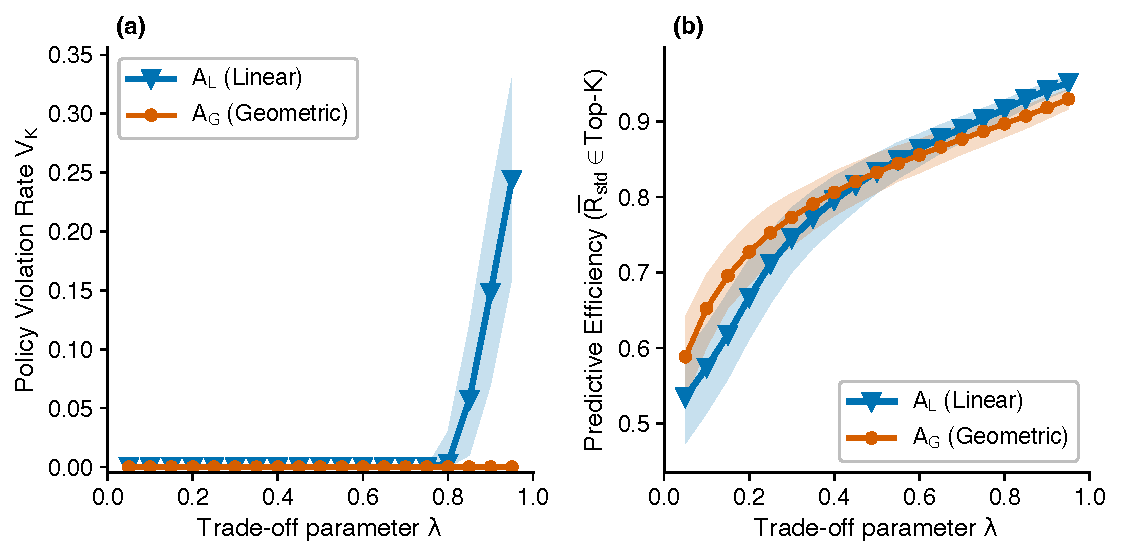
\includegraphics[width=\textwidth]{figures/opportunity_cost.pdf}
\caption{{\color{red}Policy compliance analysis ($N=1000$ Monte Carlo trials). Solid curves represent Monte Carlo means and shaded regions denote 95\% confidence intervals. (\textbf{a}) Policy violation rate ($\bar{V}_K$) as a function of $\lambda$. (\textbf{b}) Average predictive score ($\bar{R}_K$) of the selected non-vetoed Top-$K$ alternatives.}}
\label{fig:opportunity_cost}
\end{figure}

{\color{red}
The linear operator exhibits a clear compliance limit. As $\lambda$ increases, the average predictive score of the selected alternatives improves steadily while policy compliance is preserved. Specifically, $A_L$ maintains $\bar{V}_K=0$ up to approximately $\lambda=0.75$ (95\% CI upper bound), during which $\bar{R}_K$ increases from about $0.53$ to $0.90$. Beyond this point, however, contextually excluded alternatives begin to enter the prioritized tier. At $\lambda=0.95$, approximately 24\% of the Top-$K$ alternatives belong to the veto group ($\bar{V}_K\approx0.24$, 95\% CI $[0.16,0.33]$), despite achieving an average predictive score close to $0.95$.
}

{\color{red}This behavior is consistent with Corollary~\ref{cor:linear_reversal} for the linear family: sufficiently large predictive scores compensate for a zero context score, allowing contextually excluded alternatives to enter the prioritized set once the predictive component dominates the aggregation.}

The weighted geometric operator behaves differently. Because $Q_i=0$ always implies $P_i=0$, policy compliance is preserved throughout the entire range of $\lambda$, with $\bar{V}_K=0$ in all Monte Carlo trials. At the same time, the average predictive score continues to increase as $\lambda$ grows, reaching values comparable to those obtained with the linear operator without admitting contextually excluded alternatives.

Overall, these results show that the limitation of linear aggregation is not its ability to exploit the predictive score at moderate values of $\lambda$, but its inability to preserve both high predictive scores and full policy compliance when prediction becomes the dominant component of the prioritization. In contrast, the weighted geometric operator extends the range of admissible $\lambda$ values over which both objectives can be achieved simultaneously.

\subsection{Robustness to Predictive Overconfidence}
\label{subsect:firewall}

This experiment evaluates how localized predictive overconfidence affects policy compliance. Specifically, predictive scores within the veto group are progressively increased while their context scores remain fixed at $Q_i=0$, allowing us to assess whether artificially inflated predictive scores can promote contextually excluded alternatives into the Top-$K$ tier. 

 As noted in Table~\ref{tab:sim_protocol}, predictive overconfidence is modeled through the parameter $\mu_{\text{shift}}$, which controls the mean predictive score assigned to the veto subgroup. Specifically, predictive scores for vetoed alternatives are generated from $R_i \sim \mathcal{N}(\mu_{\text{shift}},0.05^2)$,
truncated to the interval $[0,1]$. Increasing $\mu_{\text{shift}}$ therefore simulates progressively more adverse scenarios in which the predictive subsystem systematically assigns high scores to alternatives that should ultimately be rejected by the contextual layer.

The trade-off parameter is fixed at $\lambda=0.85$, where the predictive score has sufficient influence for compensatory effects to emerge. Lower values of $\lambda$ would cap the priority score of vetoed alternatives below the empirical Top-$K$ threshold, masking the differences between aggregation operators.

Figure~\ref{fig:predictive_overconfidence} reports the policy violation rate ($\bar{V}_K$) as the mean predictive score of the veto group increases.
{\color{red}
The linear operator remains fully compliant while the predictive scores of the veto group are moderate. However, once their average predictive score exceeds approximately $0.85$, policy violations increase steadily. At $\mu_{\text{shift}}=1.0$, nearly 29\% of the prioritized Top-$K$ alternatives belong to the veto group ($\bar{V}_K\approx0.29$, 95\% CI $[0.14,0.44]$). This behavior indicates that sufficiently large predictive scores compensate for the absence of contextual support, allowing contextually excluded alternatives to enter the prioritized set.
}

\begin{figure}[t]
\centering
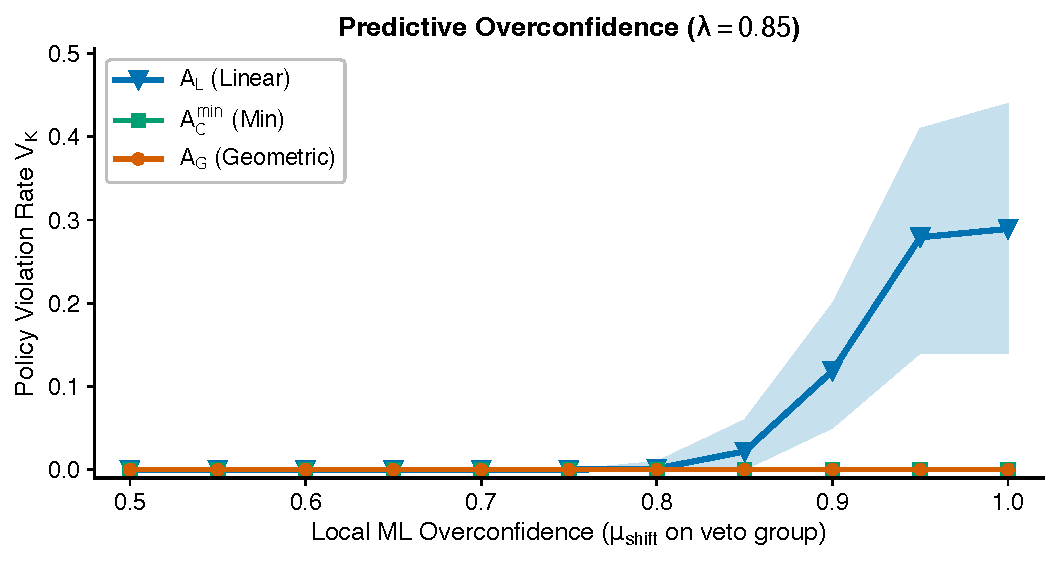
\includegraphics[width=\textwidth]{figures/predictive_overconfidence.pdf}
\caption{{\color{red}Robustness to predictive overconfidence ($\lambda=0.85$, $N=1000$ Monte Carlo trials). Solid curves represent Monte Carlo means and shaded regions denote 95\% confidence intervals. The horizontal axis controls the mean predictive score assigned to the veto group. The vertical axis reports the policy violation rate ($\bar{V}_K$).}}
\label{fig:predictive_overconfidence}
\end{figure}

By contrast, both the minimum and weighted geometric operators maintain $\bar{V}_K=0$ throughout the entire range of predictive shifts. Since $Q_i=0$ always implies $P_i=0$, increasing the predictive score alone cannot promote vetoed alternatives into the Top-$K$ tier.

{\color{red}These results are consistent with Theorem~\ref{thm:veto} for the non-compensatory family (minimum) and with Corollary~\ref{cor:geom_reversal} for the geometric mean: the veto property prevents any positive predictive score from overriding a null contextual evaluation.}

{\color{red}
\subsection{Compensation Limits under Intermediate Context}
\label{subsect:intermediate_context}

The previous experiments focus on hard contextual exclusions ($Q_i=0$), for which zero-absorption already implies that non-linear operators exclude the affected alternatives. To address settings in which the algebraic implication is less immediate, we next consider an intermediate-context regime. Specifically, a subgroup $X_{\mathrm{inter}}$ (20\% of the population) is assigned a fixed moderate context score $Q_i=0.5$ together with artificially high predictive scores $R_i\sim\mathcal{N}(0.9,0.05^2)$, while the remaining candidates are drawn uniformly in $(R_i,Q_i)$. The evaluation metric is the acceptance rate of $X_{\mathrm{inter}}$ into the Top-$K$ tier as $\lambda$ is swept from $0.1$ to $0.9$.

This design isolates a compensation question that cannot be reduced to zero absorption: can a strong predictive recommendation override a merely mediocre contextual assessment? Corollary~\ref{cor:linear_reversal} predicts that the linear family admits such overrides once the predictive weight is large enough relative to the context gap, because compensation enters additively through $\Phi_{A_L}$. By contrast, Corollary~\ref{cor:geom_reversal} implies a relative (logarithmic) threshold for $A_G$: reversing a balanced competitor requires a proportionally larger contextual improvement, so an imbalance between $R\approx 0.9$ and $Q=0.5$ is penalized more severely under sub-compensatory aggregation.

Figure~\ref{fig:intermediate_context} reports the Monte Carlo acceptance curves. Under $A_L$, candidates from $X_{\mathrm{inter}}$ begin to enter the prioritized tier around $\lambda\approx 0.50$ and the acceptance rate rises steeply thereafter, reaching approximately $0.48$ at $\lambda=0.9$. Inflated predictive scores therefore compensate for the mediocre context early, flooding the Top-$K$ boundary once prediction dominates the linear mix.

The weighted geometric operator responds more cautiously. Acceptance remains near zero until about $\lambda\approx 0.55$ and only then increases, remaining systematically below the linear curve over the mid-range of $\lambda$ (for example, $\bar{0.19}$ vs.\ $\bar{0.08}$ at $\lambda=0.6$). This delay is consistent with the sub-compensatory semantics of $A_G$: the same high-$R$/moderate-$Q$ imbalance is discounted until the predictive exponent becomes large, so a higher $\lambda$ is required before $X_{\mathrm{inter}}$ systematically overtakes candidates with more balanced scores. At the upper end of the sweep the two curves converge, confirming that the distinction is most informative in the intermediate compensation regime rather than at extreme predictive dominance.

\begin{figure}[t]
\centering
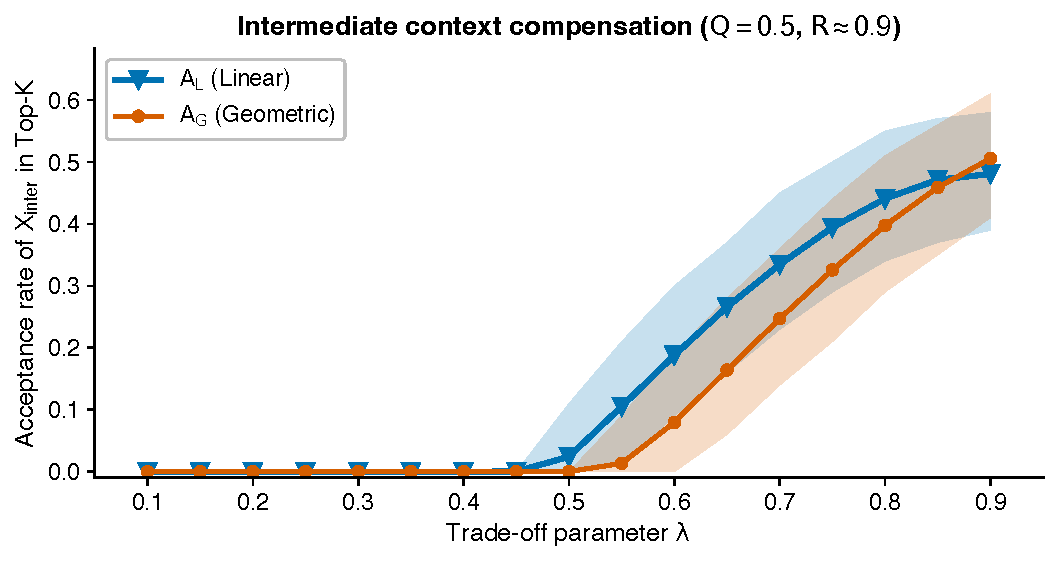
\includegraphics[width=\textwidth]{figures/intermediate_context.pdf}
\caption{{\color{red}Acceptance rate of candidates with intermediate context ($Q=0.5$) but high predictive scores ($R \approx 0.9$) into the Top-$K$ tier ($N=1000$ Monte Carlo trials). Solid curves represent Monte Carlo means and shaded regions denote 95\% confidence intervals.}}
\label{fig:intermediate_context}
\end{figure}
}

{\color{red}
\subsection{Rank Stability Under Imprecision in Context Evaluation}
\label{subsect:noise}

To ensure that the robustness claim generalizes beyond a single operating point, this experiment evaluates rank stability under an expanded factorial design: three trade-off values $\lambda\in\{0.25,0.50,0.75\}$, two population models (Uniform $\mathcal{U}(0,1)$ and Beta $\mathcal{B}(2,2)$), and two contextual perturbation laws (Gaussian $\mathcal{N}(0,\sigma^2)$ and Uniform $\mathcal{U}(-\sigma,\sigma)$ with $\sigma\in[0,0.5]$), yielding twelve settings per Monte Carlo trial ($N=1000$). We report $\bar{\tau}(\sigma)$ and $J_K(\sigma)$ as defined above.

Figure~\ref{fig:noise_propagation} summarizes the results averaged over population model and perturbation law. At $\sigma=0.5$, the minimum operator ($A_C^{\min}$) consistently achieves higher Top-$K$ overlap than the linear operator ($A_L$) for $\lambda\le 0.50$. For example, at $\lambda=0.25$ the mean Jaccard index is approximately $0.38$ for $A_C^{\min}$ (95\% CI $[0.30,0.46]$) versus $0.25$ for $A_L$ (95\% CI $[0.19,0.32]$), and this ordering holds in every individual configuration of population model and noise law. At $\lambda=0.50$, $A_C^{\min}$ again maintains higher tier overlap ($\bar{J}_K\approx 0.38$ vs.\ $\bar{J}_K\approx 0.35$), whereas global Kendall correlation becomes comparable. When $\lambda=0.75$, predictive dominance reduces the differential impact of contextual perturbations and $A_L$ exhibits higher global correlation ($\bar{\tau}\approx 0.77$ vs.\ $\bar{\tau}\approx 0.49$), reflecting that rank stability under imprecision is itself $\lambda$-dependent rather than operator-invariant.

These patterns are consistent with Theorem~\ref{thm:homog_preserv}. Under linear aggregation, every perturbation in the context score contributes directly to the priority score, so imprecision propagates throughout the ranking. In contrast, the minimum operator is affected only when the perturbed context score becomes the limiting component. Whenever $R_i\le Q_i+\epsilon$, the aggregated score remains equal to $R_i$, providing a structural buffer that preserves both global ordering and, more importantly for policy compliance, the composition of the Top-$K$ tier under moderate contextual uncertainty.

\begin{figure}[H]
\isPreprints{}{% This command is only used for ``preprints''.
\begin{adjustwidth}{-\extralength}{0cm}
\centering
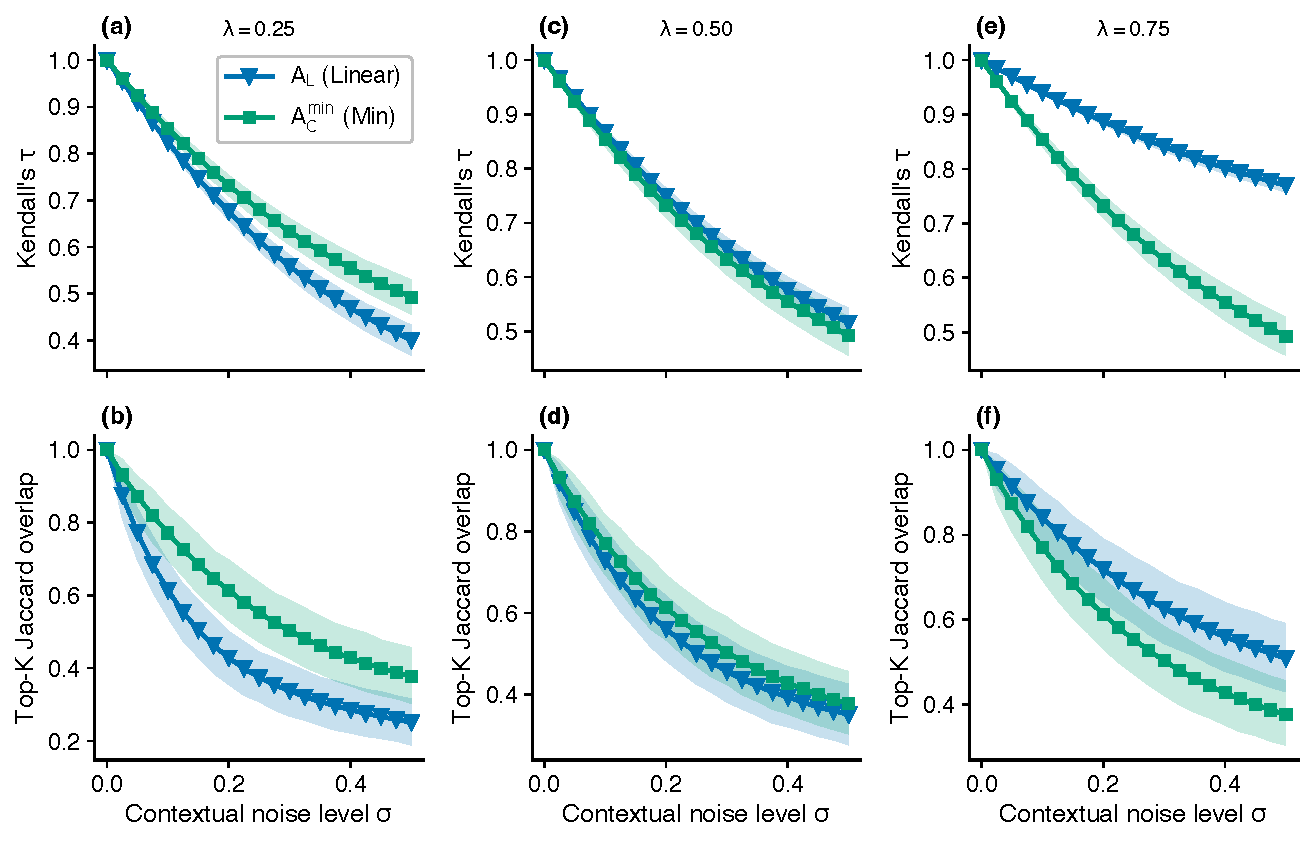
\includegraphics[width=0.9\fulllength]{figures/noise_propagation.pdf}
\caption{Rank stability and Top-$K$ overlap across multiple $\lambda$ regimes and noise models ($N=1000$ Monte Carlo trials). Top row: Kendall's $\bar{\tau}(\sigma)$; bottom row: Top-$K$ Jaccard overlap. Columns correspond to $\lambda\in\{0.25,0.50,0.75\}$. Curves are averaged over Uniform/Beta populations and Gaussian/Uniform perturbations; shaded regions denote 95\% empirical confidence intervals.}
\label{fig:noise_propagation}
\isPreprints{}{% This command is only used for ``preprints''.
\end{adjustwidth}
} % If the paper is ``preprints'', please uncomment this parenthesis.
% \end{adjustwidth}
\end{figure}
}

Together with the previous experiments, these results show that the choice of aggregation operator influences not only the balance between prediction and context, but also the robustness of the resulting prioritization. While the linear operator performs well within a limited range of $\lambda$ for compliance-oriented objectives, the minimum operator preserves contextual constraints and exhibits greater stability of the Top-$K$ tier under contextual imprecision, particularly when the context component retains substantial weight in the aggregation.

\section{Analysis in a Realistic Case Study}
\label{sect:real_example}

The previous experimental analysis isolated the behavior of the aggregation operators under controlled conditions. We now examine whether similar patterns are observed in a realistic CADEMAS-ML application using the employee attrition case study introduced by \citet{Godz2026}. The analysis considers the complete cohort of $n=100$ employees and a resource-constrained intervention policy selecting the Top-$K$ alternatives with $K=10$. Each employee is represented directly by a predictive score $R_i$ and a context score $Q_i$, obtained from the original CADEMAS-ML workflow.

The predictive score aggregates the outputs of the cooperative ADM units, whereas the context score represents the degree of alignment of an employee with the \textit{Digital Transformation} context. In this cohort, $R_i\in[0.001,0.989]$, $Q_i\in[0,0.73]$, and 35 employees receive $Q_i=0$, corresponding to contextually excluded cases. The observed attrition label in the original dataset is retained only for validation and does not participate in the prioritization process.

Five integration settings are compared: the linear operator $A_L$ with $\lambda=\{0.1,0.5,0.9\}$, together with the minimum ($A_C^{\min}$) and weighted geometric ($A_G$) operators. Particularly, for $A_G$ we employed $\lambda=0.5$. Table~\ref{tab:real_example} summarizes the Top-$K$ employees obtained under the five integration settings, whereas Figures~\ref{fig:real_example_plane} and~\ref{fig:real_example_bump} provide complementary visualizations of the employee distribution in the $(Q_i,R_i)$ space and the corresponding rank evolution across operators. Names are fictitious and are used only to facilitate the discussion of representative cases.

\begin{table}[H]
    \isPreprints{}{% This command is only used for ``preprints''.
\begin{adjustwidth}{-\extralength}{0cm}}
    \caption{Top-$K$ employees across the five integration settings for the 100-employee attrition cohort (Digital Transformation scenario, $K=10$). The first block lists the baseline Top-$K$ tier under $A_L$ with $\lambda=0.5$; the second block lists employees who enter the Top-$K$ tier under at least one alternative operator. In the baseline block, plain $P_i$ values denote Top-$K$ membership and bold values mark exclusion; in the second block, bold italic values mark entry under the corresponding operator.}
    \label{tab:real_example}
    \renewcommand{\arraystretch}{1.3}\scriptsize
    \centering
    \begin{tabularx}{\fulllength}{>{\raggedright\arraybackslash}p{2.4cm}|>{\raggedright\arraybackslash}l|R|R|R|R|R|R|R|C}
    \toprule
    \textbf{Group} & \textbf{Employee} & $R_i$ & $Q_i$ & $P_i^{(L,0.1)}$ & $P_i^{(L,0.5)}$ & $P_i^{(L,0.9)}$ & $P_i^{(C^{\min})}$ & $P_i^{(G)}$ & \textbf{Attrition} \\
    \midrule
    \multirow[m]{10}{*}{\shortstack{Baseline Top-$K$\\($A_L$, $\lambda=0.5$)}} & Laura Baker & 0.9359 & 0.6000 & 0.6336 & 0.7679 & 0.9023 & 0.6000 & 0.7493 & Yes \\
    & Andrew Wood & 0.9288 & 0.5667 & 0.6029 & 0.7477 & 0.8925 & 0.5667 & 0.7255 & Yes \\
    & Alice Brown & 0.9295 & 0.5600 & 0.5969 & 0.7447 & 0.8925 & 0.5600 & 0.7215 & Yes \\
    & Andrew Ross & 0.9302 & 0.4667 & 0.5130 & 0.6984 & \textbf{0.8839} & 0.4667 & 0.6589 & Yes \\
    & Caroline Bennett & 0.9368 & 0.4571 & 0.5051 & 0.6970 & \textbf{0.8888} & 0.4571 & 0.6544 & Yes \\
    & Jessica Wilson & 0.9444 & 0.4000 & \textbf{0.4544} & 0.6722 & \textbf{0.8900} & 0.4000 & 0.6146 & Yes \\
    & Noah Murphy & 0.9743 & 0.3600 & \textbf{0.4214} & 0.6672 & 0.9129 & 0.3600 & 0.5923 & Yes \\
    & Eleanor Foster & 0.9574 & 0.3333 & \textbf{0.3957} & 0.6454 & 0.8950 & 0.3333 & 0.5649 & Yes \\
    & Christian Bennett & 0.9690 & 0.3200 & \textbf{0.3849} & 0.6445 & 0.9041 & \textbf{0.3200} & \textbf{0.5569} & Yes \\
    & Madison Foster & 0.9193 & 0.3667 & \textbf{0.4219} & 0.6430 & \textbf{0.8641} & 0.3667 & 0.5806 & Yes \\
    \midrule
    \multirow[m]{10}{*}{\shortstack{Top-$K$ entrants under\\alternative operators}} & Leah Cooper & 0.9611 & 0.3000 & 0.3661 & 0.6306 & \textbf{\textit{0.8950}} & 0.3000 & 0.5370 & Yes \\
    & Amelia Davis & 0.9879 & 0.2667 & 0.3388 & 0.6273 & \textbf{\textit{0.9158}} & 0.2667 & 0.5133 & Yes \\ 
    & Lucy Scott & 0.8747 & 0.3667 & 0.4175 & 0.6207 & 0.8239 & \textbf{\textit{0.3667}} & \textbf{\textit{0.5663}} & Yes \\
    & Dominic Collins & 0.9774 & 0.2000 & 0.2777 & 0.5887 & \textbf{\textit{0.8996}} & 0.2000 & 0.4421 & Yes \\
    & Camila Phillips & 0.9893 & 0.0000 & 0.0989 & 0.4947 & \textbf{\textit{0.8904}} & 0.0000 & 0.0000 & Yes \\
    & Julia Smith & 0.0048 & 0.7333 & \textbf{\textit{0.6605}} & 0.3691 & 0.0776 & 0.0048 & 0.0592 & No \\ 
    & Caroline Adams & 0.0566 & 0.6000 & \textbf{\textit{0.5457}} & 0.3283 & 0.1109 & 0.0566 & 0.1842 & Yes \\
    & Caroline Roberts & 0.0203 & 0.6000 & \textbf{\textit{0.5420}} & 0.3102 & 0.0783 & 0.0203 & 0.1104 & No \\
    & Hunter Adams & 0.0110 & 0.5714 & \textbf{\textit{0.5154}} & 0.2912 & 0.0671 & 0.0110 & 0.0794 & No \\
    & Claire Bailey & 0.0282 & 0.5333 & \textbf{\textit{0.4828}} & 0.2808 & 0.0787 & 0.0282 & 0.1227 & No \\
    \bottomrule 
    \end{tabularx}
    \isPreprints{}{% This command is only used for ``preprints''.
	\end{adjustwidth}
    } % If the paper is ``preprints'', please uncomment this parenthesis.
    %\end{adjustwidth}
    %\noindent{\footnotesize \textbf{Bold italic} $P_i$ values: employee enters the Top-$K$ tier under the corresponding operator (second block only). \textbf{Bold} $P_i$ values: employee in the baseline block is excluded from that Top-$K$ tier.}
    \end{table}

\begin{figure}[H]
\centering 
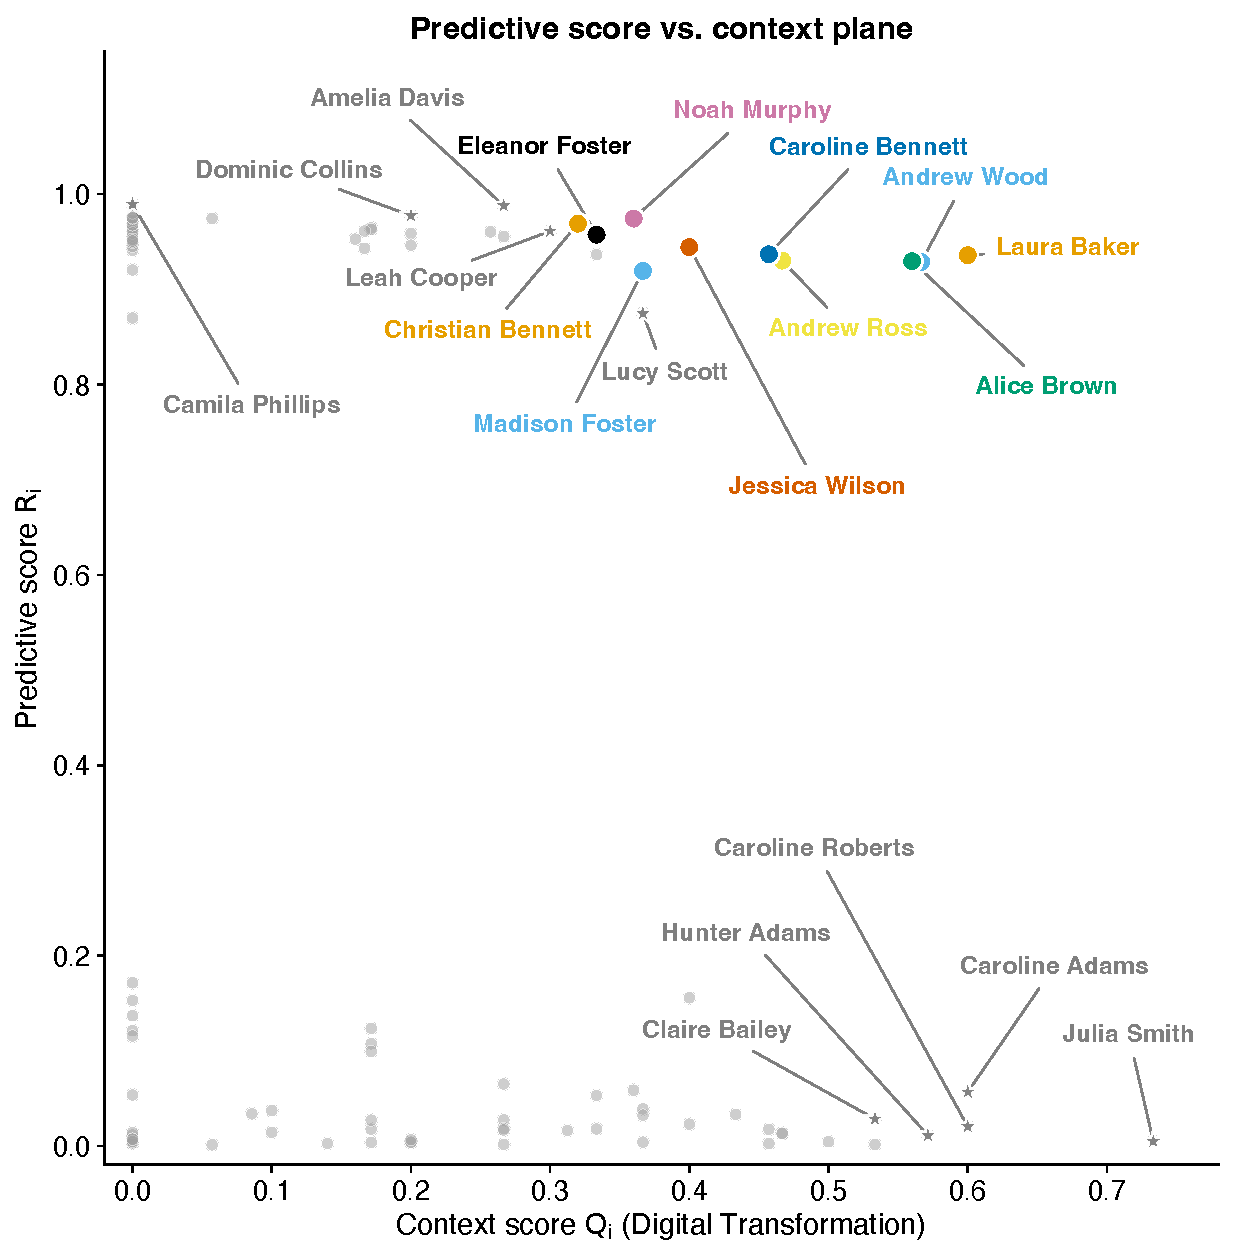
\includegraphics[width=\textwidth]{figures/real_example_plane.pdf}
\caption{Employee distribution in the predictive vs. context space. Grey points represent the complete cohort ($n=100$). Colored circles indicate the baseline Top-$K$ tier obtained with the linear operator ($A_L$, $\lambda=0.5$), whereas star markers denote employees entering the Top-$K$ tier under at least one aggregation setting.} 
\label{fig:real_example_plane} 
\end{figure} 

\begin{figure}[H]
\isPreprints{}{% This command is only used for ``preprints''.
\begin{adjustwidth}{-\extralength}{0cm}}
\centering
    %} % If the paper is ``preprints'', please uncomment this parenthesis.
\hfill
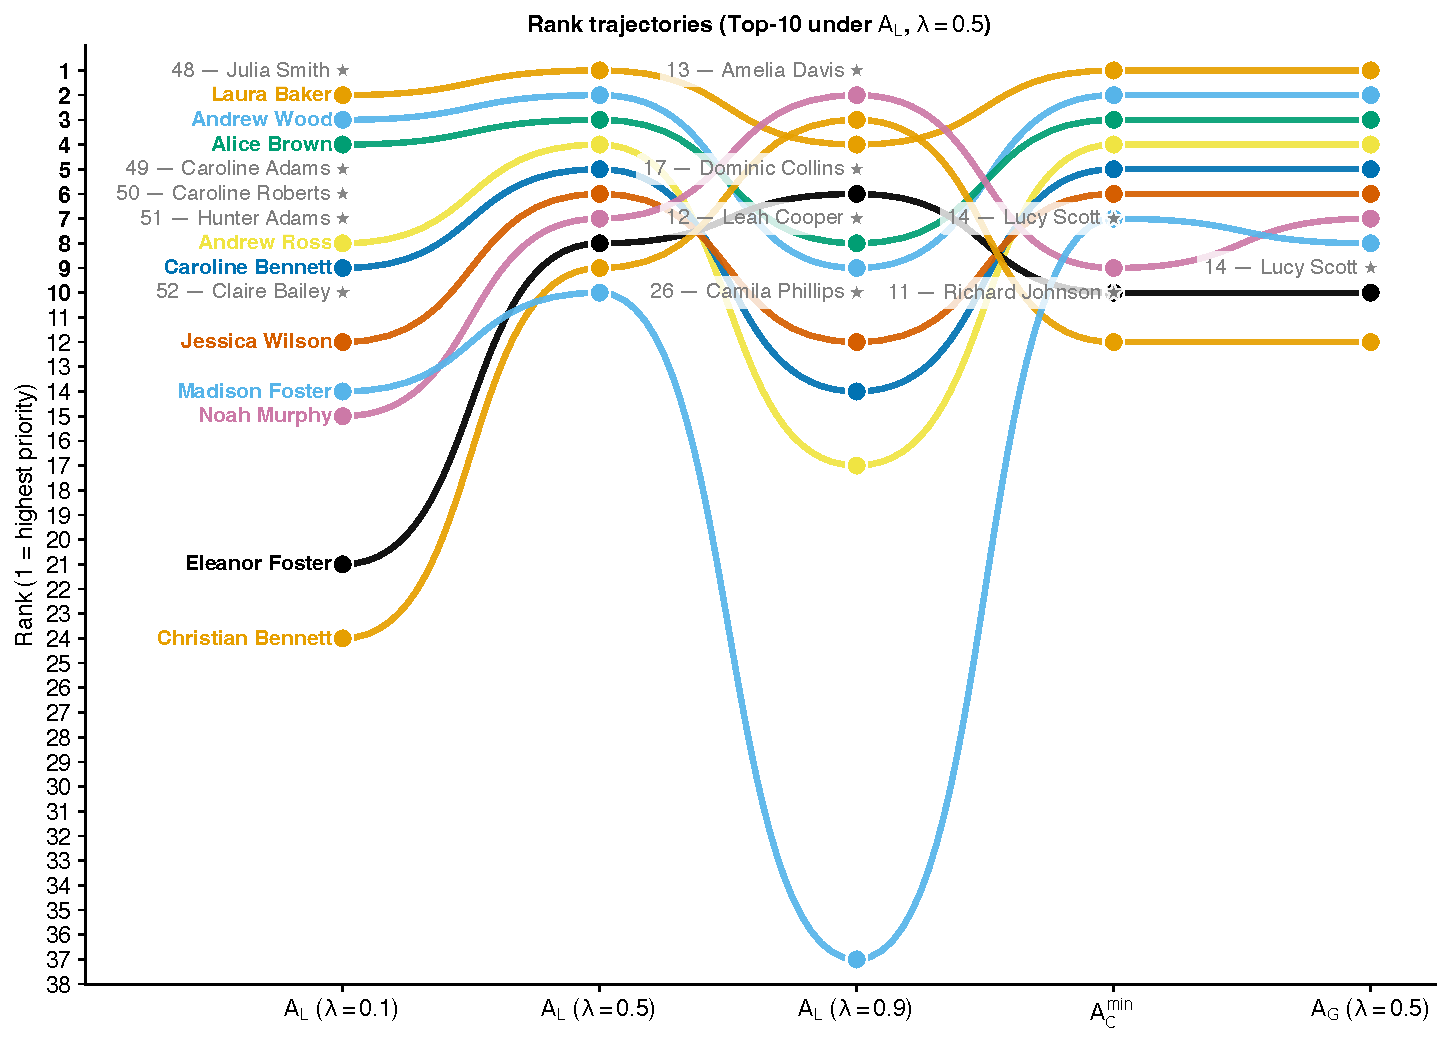
\includegraphics[width=\fulllength]{figures/real_example_bump.pdf}
\caption{Rank evolution of the baseline Top-$K$ employees across the five integration settings. Star markers denote employees entering the Top-$K$ tier under an alternative operator or parameter setting. For these additional employees, the numeric prefix in the label indicates their rank in the baseline configuration ($A_L$, $\lambda=0.5$).}
\label{fig:real_example_bump}
\isPreprints{}{% This command is only used for ``preprints''.
\end{adjustwidth}
} % If the paper is ``preprints'', please uncomment this parenthesis.
% \end{adjustwidth}
\end{figure} 

The results in Table~\ref{tab:real_example} show that decreasing $\lambda$ shifts the linear operator toward a progressively more context-driven prioritization. Employees with strong contextual alignment but only modest predictive scores move upward in the ranking, even when their estimated attrition risk is low. The most extreme example is Julia Smith, whose context score is the highest in the cohort ($Q_i=0.733$) but whose predictive score is only $R_i=0.005$. Under the baseline configuration ($A_L$, $\lambda=0.5$), she ranks 48th, yet under $A_L$ with $\lambda=0.1$ she becomes the highest-priority employee. Similar behavior is observed for Caroline Adams, Caroline Roberts, Hunter Adams, and Claire Bailey, all of whom enter the Top-$K$ exclusively under the context-oriented linear configuration. Figure~\ref{fig:real_example_plane} shows that these employees occupy the upper-left region of the $(Q_i,R_i)$ plane, where strong contextual support compensates for weak predictive evidence.

Increasing $\lambda$ produces the opposite effect. As predictive evidence becomes dominant, employees with high predicted attrition risk but weak contextual alignment progressively move toward the intervention tier. Table~\ref{tab:real_example} shows that Camila Phillips, who has the highest predictive score in the cohort ($R_i=0.989$) but a null context score ($Q_i=0$), rises from rank 26 in the baseline configuration to the Top-$K$ under $A_L$ with $\lambda=0.9$. Leah Cooper, Amelia Davis, and Dominic Collins exhibit the same tendency, although with non-zero context scores. Their locations in Figure~\ref{fig:real_example_plane} correspond to the lower-right portion of the score space, illustrating how highly predictive but weakly aligned employees become increasingly favored as the predictive component receives greater weight.

The non-linear operators exhibit markedly different behavior. As shown in Table~\ref{tab:real_example}, the conjunctive minimum operator never allows employees with $Q_i=0$ to enter the prioritized set, regardless of their predictive score. The weighted geometric mean behaves less restrictively but still penalizes severe imbalance between prediction and context, preventing contextually excluded employees from reaching the intervention tier. Consequently, both operators preserve the contextual constraints identified in the theoretical analysis, whereas the linear operator eventually overrides them for sufficiently large values of $\lambda$.

The minimum operator also introduces a characteristic behavior absent from the compensatory schemes. Because the aggregated score is determined by the limiting component, different employees frequently receive identical priority values, producing ties in the final ranking. This effect is visible in Table~\ref{tab:real_example}, where several employees share exactly the same aggregated score under $A_C^{\min}$, and becomes more apparent in the rank trajectories of Figure~\ref{fig:real_example_bump}, where groups of employees collapse onto the same ranking level. Such ties are a direct consequence of the conjunctive semantics of the minimum operator rather than an artifact of the dataset.

Finally, Figure~\ref{fig:real_example_bump} provides a global view of how the Top-$K$ tier evolves across integration settings. The baseline employees remain relatively stable under moderate changes of $\lambda$, whereas larger shifts in the integration semantics produce selective replacements rather than a complete reordering of the prioritized set. Employees entering the Top-$K$ originate from the extremes of the $(Q_i,R_i)$ plane shown in Figure~\ref{fig:real_example_plane}: highly contextual but weakly predictive employees are favored by context-oriented linear integration, whereas highly predictive but weakly contextual employees emerge only under prediction-oriented linear integration. In contrast, both non-linear operators substantially reduce these extreme transitions by enforcing stronger interaction between predictive evidence and contextual assessment.

Overall, the realistic case study confirms the theoretical and simulation results. Linear aggregation behaves as a continuously adjustable compromise between prediction and context, while the minimum and weighted geometric operators encode fundamentally different integration policies that cannot be reproduced by merely tuning $\lambda$. Consequently, the choice of aggregation operator has a direct and practically significant impact on which employees ultimately receive intervention priority.

\section{Conclusions and Future Directions}\label{sect:conclusions}

This paper investigated how the aggregation operator shapes the integration of predictive and contextual information within CADEMAS, a general framework for cooperative automated decision-making \citep{NovoaHernandez2026}. Rather than treating aggregation as a purely mathematical operation, we showed that different operators encode different decision semantics and therefore lead to different prioritization behaviors.

The theoretical analysis established the conditions under which contextual information can modify or preserve the predictive ordering of alternatives. The experimental study demonstrated that these properties have practical consequences. Linear aggregation provides a flexible trade-off between predictive and context scores, but may allow contextually excluded alternatives to enter the prioritized set when the predictive component dominates the aggregation. In contrast, the minimum and weighted geometric operators preserve contextual exclusions while exhibiting greater robustness to localized predictive overconfidence and to imprecision in the context scores. The employee attrition case study confirmed that these behaviors remain visible in a realistic CADEMAS-ML application, illustrating how the choice of aggregation operator directly influences the final intervention priorities.

These results suggest that the aggregation operator should be regarded as a fundamental design choice in cooperative decision-making systems rather than as an implementation detail. Different organizations may attach different meanings to the context score: in some applications it represents guidance that can be balanced against predictive evidence, whereas in others it represents requirements that should not be compensated by high predictive scores. Selecting an aggregation operator therefore amounts to selecting the decision semantics through which predictive evidence and contextual knowledge interact.

This work has several limitations. The simulation study relies on synthetic populations designed to isolate individual behaviors of the aggregation operators rather than reproduce the full complexity of real applications. The case study uses precomputed predictive and context scores from an existing CADEMAS-ML instantiation instead of retraining the underlying predictive models. In addition, the analysis considers a representative subset of aggregation operators and focuses on ranking-based prioritization under resource constraints, without addressing issues such as fairness, intervention costs, or temporal adaptation of predictive models.

Future work will extend this analysis in several directions. An immediate step is to evaluate the proposed methodology on different application domains and with larger real-world cohorts. It will also be valuable to study broader families of aggregation operators, including parameterized fuzzy connectives and MCDM aggregation schemes, to better understand how different decision semantics influence prioritization. Another promising direction is to incorporate application-specific utility and cost models so that aggregation strategies can be evaluated not only by their ranking behavior but also by their practical consequences. Finally, and in the context of CADEMAS-ML, it is clear that  aggregation strategies should be considered as configurable components, allowing domain experts to explore their impact on policy compliance, prioritization, and decision robustness during system design.

%%%%%%%%%%%%%%%%%%%%%%%%%%%%%%%%%%%%%%%%%%
\authorcontributions{All authors contributed equally to this work. All authors have read and agreed to the published version of the manuscript.}

\funding{This research was supported by the project ``Study, Analysis and Evaluation of Cooperative Automated Decision-Making Systems (CADEMAS)'', PID2023-146575NB-I00, funded by MCIU/AEI/I0.13039/501100011033 and by FSE+. The authors acknowledge support of the previous project.}

\institutionalreview{Not applicable.}

\informedconsent{Not applicable.} 

\dataavailability{Simulation code, figure scripts, and cohort data for the real attrition example are available in the project repository at \url{https://github.com/pnovoahe/cademas-mathematics} (\texttt{experiments/}; 100-case CADEMAS-ML cohort in \texttt{experiments/data/attrition100/}). The underlying IBM HR Analytics dataset is publicly available on Kaggle.} 

\acknowledgments{Mariia Godz has a pre-doctoral research contract associated with the project ``Study, Analysis and Evaluation of Cooperative Automated Decision-Making Systems (CADEMAS)'', PID2023-146575NB-I00, funded by MCIU/AEI/I0.13039/501100011033 and by FSE+. The authors acknowledge support of the previous project.}

\conflictsofinterest{The authors declare no conflicts of interest.}


%%%%%%%%%%%%%%%%%%%%%%%%%%%%%%%%%%%%%%%%%%
%\isPreprints{}{% This command is only used for ``preprints''.
\begin{adjustwidth}{-\extralength}{0cm}
%} % If the paper is ``preprints'', please uncomment this parenthesis.
%\printendnotes[custom] % Un-comment to print a list of endnotes

\reftitle{References}
%\bibliography{biblio.bib}

\begin{thebibliography}{999}
    
    \bibitem[Kierner et~al.(2023)Kierner, Kucharski, and Kierner]{Kierner2023}
    Kierner, S.; Kucharski, J.; Kierner, Z.
    \newblock Taxonomy of Hybrid Architectures Involving Rule-Based Reasoning and
    Machine Learning in Clinical Decision Systems: A Scoping Review.
    \newblock {\em Journal of Biomedical Informatics} {\bf 2023}, {\em
        144},~104428.
    \newblock {\url{https://doi.org/10.1016/j.jbi.2023.104428}}.
    
    \bibitem[Rahman et~al.(2025)Rahman, Zainal, Mubarak, Shabir, Anwar, and
    Asrowardi]{Rahman2025}
    Rahman, T.; Zainal, D.; Mubarak, H.; Shabir, F.; Anwar, N.; Asrowardi, I.
    \newblock Utilizing Machine Learning-Based Decision-Making to Align Higher
    Education Curriculum with Industry Requirements.
    \newblock {\em International Journal of Modern Education and Computer Science}
    {\bf 2025}, {\em 17},~1--15.
    \newblock {\url{https://doi.org/10.5815/ijmecs.2025.04.01}}.
    
    \bibitem[Pérez-Domínguez et~al.(2024)Pérez-Domínguez, Callejas-Cuervo, and
    García-Luna]{PerezDominguez2024}
    Pérez-Domínguez, L.; Callejas-Cuervo, M.; García-Luna, F.
    \newblock Intuitionistic Fuzzy Dimensional Analysis in Multi-Criteria
    Decision-Making: A Computational Approach.
    \newblock {\em IEEE Access} {\bf 2024}, {\em 12},~1--15.
    \newblock {\url{https://doi.org/10.1109/ACCESS.2024.3422616}}.
    
    \bibitem[Novoa-Hernández et~al.(2026)Novoa-Hernández, Pelta, Godz, Verdegay,
    and Buendia-Carrillo]{NovoaHernandez2026}
    Novoa-Hernández, P.; Pelta, D.; Godz, M.; Verdegay, J.; Buendia-Carrillo, D.
    \newblock {CADEMAS} – A Framework for Cooperative Automated Decision-Making
    Systems.
    \newblock In Proceedings of the Proceedings of the 2026 IEEE Conference on
    Artificial Intelligence (CAI),  2026, pp. 756--761.
    \newblock {\url{https://doi.org/10.1109/CAI68641.2026.11536392}}.
    
    \bibitem[{ELI Innovation Paper}(2022)]{ELI_ADM_Principles_2022}
    {ELI Innovation Paper}.
    \newblock Guiding Principles for Automated Decision-Making in the {EU}.
    \newblock Innovation paper, European Law Institute (ELI),  2022.
    
    \bibitem[Godz et~al.(2026)Godz, Novoa-Hernández, and Pelta]{Godz2026}
    Godz, M.; Novoa-Hernández, P.; Pelta, D.
    \newblock A Cooperative and Context-Aware Approach for Employee Attrition
    Prevention. In {\em Information Processing and Management of Uncertainty in
        Knowledge-Based Systems}; Springer Nature Switzerland,  2026; pp. 203--217.
    \newblock {\url{https://doi.org/10.1007/978-3-032-29000-7_15}}.
    
    \bibitem[Yager(1988)]{Yager1988}
    Yager, R.
    \newblock On Ordered Weighted Averaging Aggregation Operators in Multicriteria
    Decisionmaking.
    \newblock {\em IEEE Transactions on Systems, Man, and Cybernetics} {\bf 1988},
    {\em 18},~183--190.
    \newblock {\url{https://doi.org/10.1109/21.87068}}.
    
    \bibitem[Tan and Chen(2010)]{Tan2009}
    Tan, C.; Chen, X.
    \newblock Induced Intuitionistic Fuzzy Ordered Weighted Geometric Operator and
    Its Application to Multiple Attribute Decision Making.
    \newblock {\em International Journal of Intelligent Systems} {\bf 2010}, {\em
        25},~1193--1209.
    \newblock {\url{https://doi.org/10.1002/int.20446}}.
    
    \bibitem[Grabisch et~al.(2000)Grabisch, Murofushi, and Sugeno]{Grabisch1996}
    Grabisch, M.; Murofushi, T.; Sugeno, M.
    \newblock Aggregation Operators and Fuzzy Integrals. In {\em Fuzzy Measures and
        Integrals: Theory and Applications}; Physica-Verlag,  2000; pp. 3--41.
    
    \bibitem[Riaz et~al.(2022)Riaz, Farid, Wang, and Pamucar]{Riaz2022}
    Riaz, M.; Farid, H.; Wang, W.; Pamucar, D.
    \newblock Interval-Valued Linear Diophantine Fuzzy Frank Aggregation Operators
    with Multi-Criteria Decision-Making.
    \newblock {\em Mathematics} {\bf 2022}, {\em 10},~1811.
    \newblock {\url{https://doi.org/10.3390/math10111811}}.
    
    \bibitem[Senapati et~al.(2022)Senapati, Chen, and Yager]{Senapati2022}
    Senapati, T.; Chen, G.; Yager, R.
    \newblock Aczel--Alsina Aggregation Operators and Their Application to
    Intuitionistic Fuzzy Multiple Attribute Decision Making.
    \newblock {\em International Journal of Intelligent Systems} {\bf 2022}, {\em
        37},~1529--1551.
    \newblock {\url{https://doi.org/10.1002/int.22684}}.
    
    \bibitem[Akram et~al.(2020)Akram, Yaqoob, Ali, and Chammam]{Akram2020}
    Akram, M.; Yaqoob, N.; Ali, G.; Chammam, W.
    \newblock Extensions of Dombi Aggregation Operators for Decision Making under
    m-Polar Fuzzy Information.
    \newblock {\em Journal of Mathematics} {\bf 2020}, {\em 2020},~4739567.
    \newblock {\url{https://doi.org/10.1155/2020/4739567}}.
    
    \bibitem[Mardani et~al.(2018)Mardani, Nilashi, Zavadskas, Awang, Zare, and
    Jamal]{Mardani2018}
    Mardani, A.; Nilashi, M.; Zavadskas, E.K.; Awang, S.; Zare, H.; Jamal, N.M.
    \newblock Decision making methods based on fuzzy aggregation operators: Three
    decades review from 1986 to 2017.
    \newblock {\em International Journal of Information Technology \& Decision
        Making} {\bf 2018}, {\em 17},~391--466.
    \newblock {\url{https://doi.org/10.1142/S021962201830001X}}.
    
    \bibitem[Sun et~al.(2018)Sun, Dong, and Liu]{Sun2018}
    Sun, L.; Dong, H.; Liu, A.
    \newblock Aggregation functions considering criteria interrelationships in
    fuzzy multi-criteria decision making: State-of-the-art.
    \newblock {\em IEEE Access} {\bf 2018}, {\em 6},~68104--68136.
    \newblock {\url{https://doi.org/10.1109/ACCESS.2018.2879741}}.
    
    \bibitem[Kahraman et~al.(2015)Kahraman, Onar, and Oztaysi]{Kahraman2015}
    Kahraman, C.; Onar, S.C.; Oztaysi, B.
    \newblock Fuzzy multicriteria decision-making: A literature review.
    \newblock {\em International Journal of Computational Intelligence Systems}
    {\bf 2015}, {\em 8},~637--666.
    \newblock {\url{https://doi.org/10.1080/18756891.2015.1046325}}.
    
    \bibitem[Mardani et~al.(2015)Mardani, Jusoh, and Zavadskas]{Mardani2015}
    Mardani, A.; Jusoh, A.; Zavadskas, E.K.
    \newblock Fuzzy multiple criteria decision-making techniques and applications
    -- Two decades review from 1994 to 2014.
    \newblock {\em Expert Systems with Applications} {\bf 2015}, {\em
        42},~4126--4148.
    \newblock {\url{https://doi.org/10.1016/j.eswa.2015.01.003}}.
    
    \bibitem[Petrovic et~al.(2023)Petrovic, Mihajlović, Markovic,
    Hashemkhani~Zolfani, and Madić]{Petrovic2023}
    Petrovic, G.S.; Mihajlović, J.; Markovic, D.; Hashemkhani~Zolfani, S.; Madić,
    M.
    \newblock Comparison of aggregation operators in the group decision-making
    process: A real case study of location selection problem.
    \newblock {\em Sustainability} {\bf 2023}, {\em 15},~8229.
    \newblock {\url{https://doi.org/10.3390/su15108229}}.

    \bibitem[Afzal et~al.(2018)Afzal, Ali, Ali, Hussain, Ali, Khan, Amin, Kang,
    and Lee]{Afzal2018}
    Afzal, M.; Ali, S.I.; Ali, R.; Hussain, M.; Ali, T.; Khan, W.A.; Amin, M.B.;
    Kang, B.H.; Lee, S.
    \newblock Personalization of wellness recommendations using contextual
    interpretation.
    \newblock {\em Expert Systems with Applications} {\bf 2018}, {\em
        96},~506--521.
    \newblock {\url{https://doi.org/10.1016/j.eswa.2017.11.006}}.

    \bibitem[Shyur(2025)]{Shyur2025}
    Shyur, H.J.
    \newblock Combination weighting method using Z-numbers for multi-criteria
    decision-making.
    \newblock {\em Applied Soft Computing} {\bf 2025}, {\em 174},~112992.
    \newblock {\url{https://doi.org/10.1016/j.asoc.2025.112992}}.
    
    \bibitem[P{\'{e}}rez-Ca{\~{n}}edo et~al.(2023)P{\'{e}}rez-Ca{\~{n}}edo, Porras,
    Pelta, and Verdegay]{PerezCanedo2022}
    P{\'{e}}rez-Ca{\~{n}}edo, B.; Porras, C.; Pelta, D.A.; Verdegay, J.L.
    \newblock Modeling Contexts as Fuzzy Propositions in Optimization Problems.
    \newblock {\em {IEEE} Transactions on Fuzzy Systems} {\bf 2023}, {\em
        31},~1474--1483.
    \newblock {\url{https://doi.org/10.1109/tfuzz.2022.3203786}}.
    
    \bibitem[Pérez-Cañedo et~al.(2024)Pérez-Cañedo, Novoa-Hernández, Porras,
    Pelta, and Verdegay]{PerezCanedo2024}
    Pérez-Cañedo, B.; Novoa-Hernández, P.; Porras, C.; Pelta, D.A.; Verdegay,
    J.L.
    \newblock Contextual analysis of solutions in a tourist trip design problem: A
    fuzzy logic-based approach.
    \newblock {\em Applied Soft Computing} {\bf 2024}, {\em 154},~111351.
    \newblock {\url{https://doi.org/10.1016/j.asoc.2024.111351}}.
    
    \bibitem[Zimmermann and Zysno(1980)]{Zimmermann1980}
    Zimmermann, H.; Zysno, P.
    \newblock Latent Connectives in Human Decision Making.
    \newblock {\em Fuzzy Sets and Systems} {\bf 1980}, {\em 4},~37--51.
    \newblock {\url{https://doi.org/10.1016/0165-0114(80)90062-7}}.
    
    \bibitem[Natoli et~al.(2024)Natoli, Feeny, Li, and Zuhair]{Natoli2024}
    Natoli, R.; Feeny, S.; Li, J.; Zuhair, S.
    \newblock Aggregating the Human Development Index: A Non-Compensatory Approach.
    \newblock {\em Social Indicators Research} {\bf 2024}, {\em 172},~499--515.
    \newblock {\url{https://doi.org/10.1007/s11205-024-03318-7}}.
    
    \bibitem[Blancas and Contreras(2024)]{Blancas2024}
    Blancas, F.; Contreras, I.
    \newblock Global {SDG} Composite Indicator: A New Methodological Proposal That
    Combines Compensatory and Non-Compensatory Aggregations.
    \newblock {\em Sustainable Development} {\bf 2024}.
    \newblock {\url{https://doi.org/10.1002/sd.3109}}.
    
\end{thebibliography}


% If authors have biography, please use the format below
%\section*{Short Biography of Authors}
%\bio
%{\raisebox{-0.35cm}{\includegraphics[width=3.5cm,height=5.3cm,clip,keepaspectratio]{Definitions/author1.pdf}}}
%{\textbf{Firstname Lastname} Biography of first author}
%
%\bio
%{\raisebox{-0.35cm}{\includegraphics[width=3.5cm,height=5.3cm,clip,keepaspectratio]{Definitions/author2.jpg}}}
%{\textbf{Firstname Lastname} Biography of second author}

% For the MDPI journals use author-date citation, please follow the formatting guidelines on http://www.mdpi.com/authors/references
% To cite two works by the same author: \citeauthor{ref-journal-1a} (\citeyear{ref-journal-1a}, \citeyear{ref-journal-1b}). This produces: Whittaker (1967, 1975)
% To cite two works by the same author with specific pages: \citeauthor{ref-journal-3a} (\citeyear{ref-journal-3a}, p. 328; \citeyear{ref-journal-3b}, p.475). This produces: Wong (1999, p. 328; 2000, p. 475)

%%%%%%%%%%%%%%%%%%%%%%%%%%%%%%%%%%%%%%%%%%
%% for journal Sci
%\reviewreports{\\
%Reviewer 1 comments and authors’ response\\
%Reviewer 2 comments and authors’ response\\
%Reviewer 3 comments and authors’ response
%}
%%%%%%%%%%%%%%%%%%%%%%%%%%%%%%%%%%%%%%%%%%
\PublishersNote{}
%\isPreprints{}{% This command is only used for ``preprints''.
\end{adjustwidth}
%} % If the paper is ``preprints'', please uncomment this parenthesis.
\end{document}